\setcounter{chapter}{6}

\chapter{常微分方程}

由于很多问题中都涉及变量之间以及变量及其变换率之间的数量关系,
建立微分方程对其加以描述就成为了一种必要的手段。也正因为如此,
微分方程在实际问题中的应用非常广泛。

求解一些简单的常微分方程是微积分课程的一项要求,需要了解的是
可解(解析求解)的微分方程只是整个微分方程家族中极少极少的一部分。
微分方程一直以来,都被认为是数学理论中最艰深和最具挑战性的分支之一。


\section{概念与应用}

\subsection{微分方程模型}

{\bf 微分方程:}包含函数、自变量及其相关的微分项的等式。
相对于不包含任何微分项的方程,引入微分项,显然可以帮助我们描述更多的问题。

{\bf 常微分方程:} 涉及一元函数的微分方程,例如:
  $$x''(t)=a,\quad  \df{y''}{(1+y')^{3/2}}=L,\quad 
  L\df{\d i}{\d t}+Ri=E(t)$$ 
  
{\bf 偏微分方程:} 涉及多元函数的微分方程,例如:
  $$\df{\p^2U}{\p x^2}+\df{\p^2U}{\p y^2}+\df{\p^2U}{\p z^2}=0,\quad 
  \df{\p^2z}{\p x\p y}=0$$

从我们熟知和一些容易理解的问题中可以很容易地抽象出对应的微分方程模型:

{\bf 弹簧振子的运动(简谐振动):}

假设振子的质量为$1$,弹簧的质量忽略不计。以$x$表示弹簧偏离平衡位置的位移。

{\it 无阻尼的自由振动:}
$$\df{\d^2 x}{\d t^2}+k^2x=0,$$
其中$k^2$为弹簧的{\kaishu 弹性系数},理想情况下,振子运动的加速度完全
由弹簧的回复力决定,而弹簧的回复力与其变性量成正比;

{\it 带阻尼的自由振动:}
$$\df{\d^2 x}{\d t^2}+2n\df{\d x}{\d t}+k^2x=0,$$
其中$2n$为{\kaishu 阻尼系数},意味着存在一个与速度成正比的阻尼(例如:空气阻力);

{\it 带阻尼的强迫振动:}
$$\df{\d^2 x}{\d t^2}+2n\df{\d x}{\d t}+k^2x=h\sin pt$$
其中右端函数$h\sin pt$表示存在一个频率为$p$,振幅为$h$的周期性的外界作用力。

{\bf 空气中的自由落体:}

物体从一定高度开始自由下落,已知其受到的空气阻力与其速度成正比(系数$k$),
则其运动位移$S(t)$满足方程
$$S''=g-S'k$$

{\bf 追踪问题:}
某战舰发现其东北方向$(a,b)$处有一艘敌舰以速度$v_0$向正东方向行驶,于是向其发射鱼雷。
假设鱼雷的速度为$v_1\,(v_1>v_0)$,且其运动方向始终指向敌舰。试给出鱼雷运动轨迹的数学模型。

\begin{center}
	\resizebox{!}{5cm}{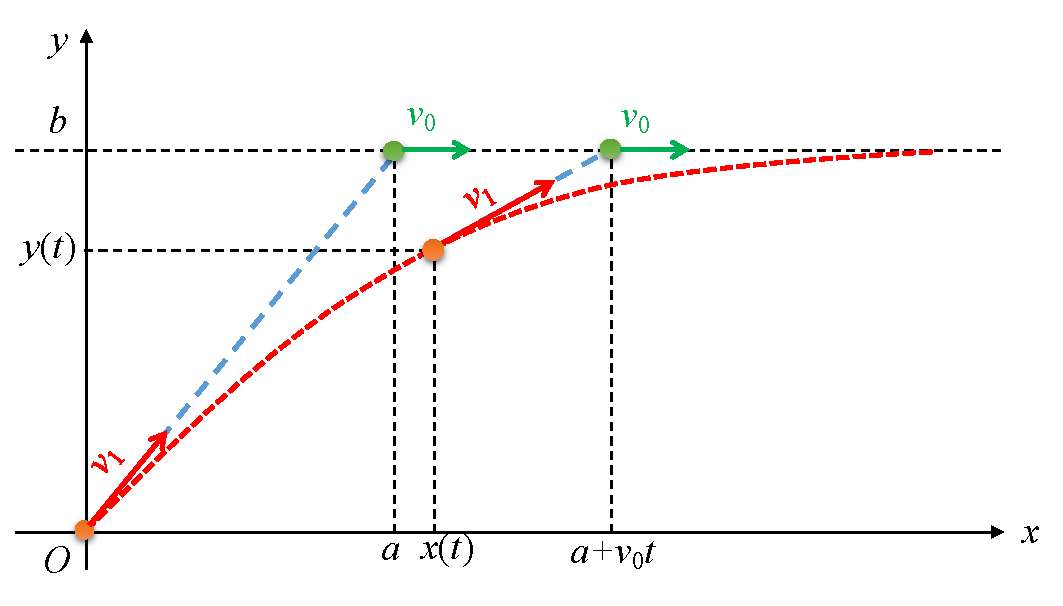
\includegraphics{./images/ch7/missile2Plane.pdf}}
\end{center}

如图,在$t$时刻,导弹走过的距离为
$$v_1t=\dint_0^x\sqrt{1+(y')^2}\d x$$
又
$$y'=\df{b-y}{a+v_0t-x}\quad\Rightarrow\quad
t=\df1{v_0}\left(\df{b-y}{y'}+x-a\right),$$
带入前式,可得
$$\df{v_1}{v_0}\left(\df{b-y}{y'}+x-a\right)=\dint_0^x\sqrt{1+(y')^2}\d
x.$$
该式两边同时对$x$求导,整理后可得
$$\df{v_1}{v_0}(y-b)y''=(y')^2\sqrt{1+(y')^2}.$$
又由题意,有$y(0)=0,\;y'(0)=b/a$。综上,导弹的轨迹应满足如下的{\kaishu 初值问题}
$$
\left\{\begin{array}{l}
\df{v_1}{v_0}(y-b)y''=(y')^2\sqrt{1+(y')^2}\\
y'(0)=b/a\\
y(0)=0
\end{array}
\right.
$$

{\bf 弱肉强食的生态系统:}
在一个生态系统中仅有两种物种$A$和$B$,其中$B$依赖于捕食$A$为生。
假设在时刻$t$二者的数量分别为$x(t)$和$y(t)$。

{\kaishu 捕食者-食饵(Predator-Prey)模型}——Lotka-Volterra Equations
$$
	\left\{\begin{array}{l}
		\df{\d x}{\d t}=ax-bxy\\
		\df{\d y}{\d t}=-cy+dxy
	\end{array}\right.
	\quad (a,b,c,d>0)
$$

其中$a,b$反映了$A,B$数量的自然变化(综合了出生率和死亡率),
$b,d$则代表了$A,B$之间的相互影响,例如:$A$越多,则$B$的食物也越多,
从而数量的增长率越高;反之,$B$越多,则被捕食的$A$也越多,从而
数量的增长率越低。

{\bf 传播模型:}

以疾病传染为例:设总人数为$N$,已感染的人数为$I$,感染率$\gamma$,
治愈率$\lambda$,则:

$$\df{\d I}{\d t}=\gamma (N-I)-\lambda I$$

类似的模型还可以用于描述信息在社会中的传播问题。

\subsection{微分方程的有关概念}

\begin{thx}
	{\bf ($n$阶)常微分方程:}形如,
	$$f(x,y,y',y'',\ldots,y^{(n)})=0,$$
	其中$y$是$x$的函数。
	\begin{enumerate}[(1)]
	  \setlength{\itemindent}{1cm}
	  \item {\bf 微分方程的解:} 使以上方程成立的函数$y=\varphi(x)$; 
	  \item {\bf 通解:}含有$n$个相互独立的任意常数的解;({\kaishu 
	  通解也即解的通用形式,因为求解$n$阶微分方程恰好需要$n$次积分,
	  因此恰好会有$n$个相互独立的积分常数})
	  \item {\bf 特解:}不存在任何未确定常数的解; 
	  \begin{itemize}
	    \item $n$阶方程的通解需包含$n$个相互独立的任意常数;
	    \item 通解有时候不代表全部的解;
	    \item {\bf 定解条件}:用来确定某个特解所需的附加条件;
	    \item 微分方程的通解表达式不唯一;
	  \end{itemize} 
	  \item {\bf 初值问题(Cauchy问题):}
	  $$
	  \left\{\begin{array}{l}
	  	f(x,y,y',y'',\ldots,y^{(n)})=0\\
	  	\quad{y^{(n-1)}(x_{n-1})=y_{n-1}}\\
	  	\quad{\ldots\ldots\ldots\ldots}\\
	  	\quad{y'(x_1)=y_1}\\
	  	\quad{y(x_0)=y_0}
	  \end{array}\right.
	  $$
	  \item {\bf 积分曲线:}微分方程的解所对应的曲线(族)。
	\end{enumerate}
\end{thx}

{\bf 例:}$y''+y=0$的两个特解$y=\sin x,\;y=\cos x$,以下为其通解的是:
\begin{enumerate}[(A)]
  \setlength{\itemindent}{1cm}
  \item $y=C_1\sin x$
  \item $y=C_1\sin x+C_2\sin x$
  \item $y=C_1\sin x+\cos(C_2x)$
  \item $y=C_1\sin x-C_2\cos x$
\end{enumerate}
进一步地,求满足$y(0)=0,\;y'(\pi)=1$的(特)解。

[解]:判定通解的条件可以归纳为:(1)满足方程(排除(C));
(2)包含两个{\kaishu 相互无关}的独立常数(排除(A)、(B)),故选(D)。

在(D)中带入$x=0$,可得$0=-C_2$,从而$y=C_1\sin x$,
$y'=C_1\cos x$,带入$x=\pi$,可得$1=-C_1$。从而所求特解为
$y=-\sin x$。\fin

\begin{shaded}
	{\bf 微分方程与积分方程}
	
	积分方程是指包含了某些积分项的方程(恒等式)。
	
	理论上,微分方程和积分方程总是可以相互转化的,例如:微分方程
	$$y'=x+y$$
	两边同时对$x$积分,可得积分方程
	$$y=\dint_0^x(x+y)\d x.$$
	同理,给定某个积分方程,总是可以通过求导,消去其中的积分运算(同时也就
	会产生一些新的导数项),化为微分方程。
	
	那么通过这样的相互转化所得到的方程等价吗?答案是否定的!原因在于{\b\it 积分方程
	通常(不是全部)都带有(隐藏的)初值条件}。例如以上的第二个方程,若令$x=0$,
	可以得到$y(0)=0$,这种条件是不可能从其对应的微分方程中得到的。
	
	因此,对于{\b 条件为积分方程的问题,务必要注意通过方程寻找可能的初值条件!}
\end{shaded}

{\bf 例:}已知某车间容积$V$,其空气中CO$_2$的密度为$\rho_1$,现以CO$_2$浓度$\rho_2(<<\rho_1)$的
新鲜空气输入,问每分钟应输入多少才能在$T$分钟后使车间中CO$_2$的含量不超过$\rho_0$。
({\bf 注:}假设新注入的空气能够与原有空气立即混合达到均匀,且空气不会被压缩。)

[提示]:$$C'=\rho_2V_1-C\df{V_1}{V},C(0)=\rho_1V$$

\begin{ext}
	{\bf 课后作业}
	\begin{enumerate}
	  \item 请给出如下通解对应的微分方程,并给出其满足给定初值条件的特解:
	  \begin{enumerate}[(1)]
	    \item $y=x^2+C_1x+C_2$,其中$C_1,C_2$为任意常数,$y(0)=y'(0)=1$; 
	    \item $y=\df{1+Ce^t}{1-Ce^t}$,其中$C$为任意常数,$y(0)=2$;
	    \item $y=(C_1+C_2x)e^x$,其中$C_1,C_2$为任意常数,$y(0)=0,y'(1)=1$;
% 	    \item $y=C_1\sin x+C_2\cos x+e^x$,其中$C_1,C_2$为任意常数,$y(0)=0,y'(\pi)=0$。
	  \end{enumerate}
	  \item 设河边点$O$的正对岸为点$A$,河宽$h$,两岸平行,水流速度恒定为$a$。
	  一只鸭子从点$A$游向点$O$,游动过程中其始终朝向$O$点。已知鸭子在
	  静水中的游速为$b(b>a)$,以$O$为原点,水流方向为$x$轴,垂直于水流
	  过河的方向为$y$轴,试给出鸭子的运动轨迹所满足的微分方程初值问题。
% 	  以$O$为坐标原点,$A$点坐标为$(0,h)$,则
% 	  $$\df{\d x}{\d y}=\df ab\sqrt{\left(\df xy\right)^2+1}-\df xy$$
% 	  初值条件$x(h)=0$
	\end{enumerate}
\end{ext}

\section{一阶微分方程的解法}

利用数学推导解析地得出微分方程的解常常是可遇不可求的,
\ps{不能解析求解的方程只能更多地依赖数值计算的方程求得
数值表示的近似解}
但确实有极少数的方程是可解的。

在所有的方程中, {\bf 一阶微分方程:}
$$f(x,y,y')=0$$
虽然并非每个都能够解析求解,但显然已经是相对最为简单的一类。
 
% \begin{itemize}
%   \item 可分离变量的方程 
%   \item 齐次方程 
%   \item 一阶线性微分方程 
%   \item Bernoulli方程
%   \item 其他可以化为以上四种形式的方程
% \end{itemize}

\subsection{可分离变量的方程}

一个方程称为是可分离变量的,是指方程经过整理后,左右两端可以分别化成
分别仅与$x$和$y$有关的形式。

\begin{thx}
	{可分离变量的方程:}
	$$\df{\d y}{\d x}=f(x)g(y)$$ 

	{\bf 解法:}若$g(y)\ne 0$,则原方程可以改写为:
	$$\df{\d y}{g(y)}=f(x)\d x,$$ 
	上式两边分别关于$x,y$求不定积分,得:
	$$\dint\df{\d y}{g(y)}=\dint f(x)\d x+C$$ 
	整理化简后既得方程的(一部分)解。结合$g(y)=0$所对应的解,即得方程全部解。
\end{thx}

{\bf 例:}求$y'=xy$的通解。
	
[解]:$y=0$显然为原方程的解。又当$y\ne0$时,原方程可化为
$$\df{\d y}y=x\d x,$$
于是
\begin{align*}
	&  \quad\d\ln|y|=\d\df12x^2,\\
	\Rightarrow\quad & \quad\ln|y|={\frac{x^2}2}+C_1\;(C_1\in\mathbb{R}),\\
	\Rightarrow\quad & \quad|y|=C_2e^{\frac{x^2}2}\;({\b C_2>0})\\
	\Rightarrow\quad & \quad y=C_3e^{\frac{x^2}2}\;({\b C_3\ne0}).
\end{align*}
综上可知,原方程的通解为
$$y=Ce^{\frac{x^2}2}\;({\b C\in\mathbb{R}}).$$\fin

{\b\it 很多时候,教材上忽略了对于分母为零的讨论,原因是分母为零对应的特解
常常可以合并到最终的通解中去,且能够使得通解的表示显得更加合理。}

{\bf 例:}求解下列微分方程\ps{如非特别说明,求解微分方程必须给出其通解!}
\begin{enumerate}[(1)]
  \setlength{\itemindent}{1cm}
%   \item $y'=xy$
  \item $\df{\d y}{\d x}=3\sin x\cos^2 y$
  \item $(e^{x+y}-e^x)\d x+(e^{x+y}+e^y)\d y=0$\hfill $(e^x+1)(e^y-1)=C$
\end{enumerate}

{\bf 注意:}分离变量时,对分母为零的情况要单独讨论!!

对于以上的(3),所得通解中无须明确地区分$x$和$y$哪一个是自变量哪一个是函数(因变量),
这种形式的通解称为{\bf 隐式通解},也是一种可以接受的通解表达形式。

{\bf 例:}已知曲线$C$上任一点$P(x,y)$处的法线与$x$轴交点为$Q$,且线段$PQ$被$y$轴平分,
求曲线$C$所满足的方程。\hfill($yy'+2x=0$)

\subsection{全微分方程}

有些情况下,求解一阶微分方程,可以通过微分运算来完成。

{\bf 例:}求解微分方程$y'=\df y\sin x$。

[解]:原方程可化为
$$\df1y\d y-\sin x\d x=0,$$
注意到$\frac1y\d y=\d\ln|y|$,$-\sin x\d x=\d\cos x$,故
上式可化为
$$\d\ln|y|+\d\cos x=0,$$
进而利用微分运算的性质(线性性),可得
$$\d(\ln|y|+\cos x)=0.$$
一个函数的微分为零,当且仅当其恒为常数,故由上式可得
$$\ln|y|+\cos x=C,\;(C\in\mbb{R}).$$
即为所求。\fin

以上的解题过程中没有直接使用积分,而是利用微分运算,最终“凑”出了
方程的通解。能够这样求解的方程被称为{\kaishu 全微分方程}\ps{全微分
方程的判定方法将在第11章的曲线积分部分加以介绍}。显然,
可分离变量的方程都是全微分方程。

{\bf 例:}求解下列方程
\begin{enumerate}[(1)]
  \setlength{\itemindent}{1cm}
  \item $(\sin x+y)\d x+(x+\cos y)\d y=0$
  \item $(e^x+e^{x+y})\d x+(e^y+e^{x+y})\d y=0$
  \item $(3y^2+2xy)\d y+(y^2+5x^4)\d x=0$
  \item $x\d x+y\d y+\df{y\d y-x\d x}{x^2+y^2}=0$
  \item $y\d x+x\d y+\df{x\d y-y\d x}{x^2+y^2}=0$
\end{enumerate}

有些情况下,一个方程虽然不是全微分方程,但可以通过乘以某个{\kaishu 积分因子},使其
变成全微分方程,例如:$x\d y-y\d x=0$就不是全微分方程,但如果方程两边都
除以$x^2$,可得
$$\df1x\d y-\df y{x^2}\d x=0,$$
进而可得
$$\df1x\d y+y\d\df1x=0,$$
利用微分运算$\d(uv)=u\d v+v\d u$,最终可得
$$\d\df yx=0,$$
进而该方程的通解为$\frac yx=C$。

求解一阶非齐次线性微分方程的常数变易法,其原理就是使用积分因子$e^{\int p(x)\d x}$,
使得方程成为了一个全微分方程(可分离变量的方程)。

\subsection{齐次方程}

{\bf 例:}
$$x^2y'=y^2,\quad y'=\df{y^2-x^2}{xy}$$ 
经过整理可分别化为
$$y'=\left(\df yx\right)^2,\quad
y'=\df{\left(\frac yx\right)^2-1}{\frac yx}.$$
也即整理后方程右端可以视为关于$\df yx$的函数。

\begin{thx}
	{\bf 齐次方程:}
	$${\b\df{\d y}{\d x}=\varphi\left(\df yx\right)}$$

	{\bf 解法:}令$z=y/x$, 则
	$$\df{\d y}{\d x}=z+x\df{\d z}{\d x},$$
	于是方程可化为
	$$\df{\d z}{\d x}=\df{\varphi(z)-z}x,$$
	这是一个可以分离变量的方程。
\end{thx}

{\bf 例:}
\begin{enumerate}[(1)]
  \setlength{\itemindent}{1cm}
  \item $y'=\df{x-y}{x+y}$\hfill $y^2+2xy-x^2=Cx^2e^{-x^2}$
  \item $(3y^2+x^2)\d y+2xy\d x=0$
  \item $\df{y}{y'}-x=\sqrt{x^2+y^2}$\hfill $y^2=2C\left(x+\df C2\right)$
\end{enumerate}

{\bf 例:}$y'=\df{2x-5y+3}{2x+4y-6}$

[提示]:令$x=X+h,y=Y+k$,带入原方程,解出$h,k$的值,使新的方程
化为齐次方程。本例中:
$$x=X+1,\;y=Y+1$$

\subsection{一阶线性微分方程}

线性微分方程是指方程中所有关于$y$和它的导数的项都是一次幂的形式,不存在
它们更高的幂次或其他的函数形式,一般地{\bf ($n$阶)线性微分方程}形如:
$$y^{(n)}+a_{n-1}(x)y^{(n-1)}+\ldots+a_1(x)y'+a_0(x)y=f(x)$$
其中$a_k(x),k=0,1,2,\ldots,n-1$和$f(x)$都是给定的函数。

\begin{thx}
	{\bf 一阶齐次线性微分方程:}
	$$y'+p(x)y=0$$
	{\bf 解法:}分离变量,通解公式:
	$${\b y=C\cdot\exp\left[-\int p(x)dx\right],\quad(C\in\mathbb{R})}$$
\end{thx}

请注意,这里的“齐次”是指方程右端恒为零,与前面介绍的齐次方程中的齐次含义有所不同。

\begin{thx}
	{\bf 一阶非齐次线性微分方程:}
	$$y'+p(x)y=q(x)$$
	{\bf 解法:}{\bf 常数变易法:}
	令齐次方程通解中的$C=C(x)$,代入非齐次方程,得
	$$\left(C(x)e^{-\int p(x)dx}\right)'+p(x)C(x)e^{-\int
	 p(x)dx}=q(x)$$
	即
	$$C'(x)e^{-\int p(x)dx}=q(x)$$
	从而
	$$C(x)=\dint q(x)e^{\int p(x)dx}dx+C_1,\quad(C_1\in\mathbb{R})$$ 
	从而得到一阶非齐次线性微分方程的通解公式:
	$${\b y=\left\{\int q(x)\exp\left[\int p(x)\d x\right]\d x+C_1\right\}
	\cdot\exp\left[-\int p(x)dx\right],\quad(C_1\in\mathbb{R})}$$
\end{thx}

常数变易法的构造思路,本质上是通过在方程两端都乘以一个所谓的{\kaishu 积分因子}
$\int p(x)\d x$,使得两端都可以表示成某个函数的导数形式
$$\b\left(ye^{\int p(x)\d x}\right)'_x=e^{\int p(x)\d x}[y'+p(x)y]
=q(x)e^{\int p(x)\d x}$$
从而间接地达到了分离变量的目的。

注:理论上,任何一个一阶方程都存在特定的积分因子,使之能够化为可分离变量的,但是
积分因子的求法往往非常复杂,并且不具有唯一性。我们更多地,是通过观察和经验
来找到特定的积分因子,在此不再详述。

{\bf 例:}$y'=\df1{x+y}$

[提示]:方程可化为
$$\df{\d x}{\d y}-x=y,$$
将$x$视为$y$的函数来求解。

\subsection{Bernoulli方程}

\begin{thx}
	{\bf Bernoulli方程:}
	$${\b y'+P(x)y=Q(x)y^n\quad(n\ne 0,1)}$$ 
	{\bf 解法:}方程两边同时除以$y^n$,得
	$$y^{-n}y'+P(x)y^{1-n}=Q(x)$$ 
	令${\b z=y^{1-n}}$,则
	$$z'+(1-n)P(x)z=(1-n)Q(x)$$
	这是一个一阶线性非齐次方程。
\end{thx}

{\bf 例:}求解下列微分方程
\begin{enumerate}[(1)]
  \setlength{\itemindent}{1cm}
  \item $y'-\df{y}{2x}=\df{x^2}{2y}$
  \item $y'=\df{x}{x^2+y^2}$\hfill$x^2+y^2+y+\df12=Ce^{2y}$
  \item $y'=xy(3+y)$\hfill$\left(Ce^{-\frac32x^2}-\df13\right)y=1$
  \item $y'=\df{x^3+y^3}{3xy^2}$\hfill$y^3=\df{x^3}2+Cx$
\end{enumerate}

\begin{shaded}
	{\bf Clairaut方程}
	$$y=xy'+f(y')$$
	两边对$x$求导,
	$$0=(x+f'(y'))y''$$
	
	{\bf 例:}求第一象限中的一条曲线,使其上每一点处的切线与两坐标轴所围三角形的
	面积等于$2$。
	
	[提示]:由题意
	$$\df12\left(x-\df y{y'}\right)(y-xy')=2,$$
	整理得
	$$y=xy'\pm2\sqrt{-y'}.$$
	解之可得
	$$y=Cx\pm2\sqrt{-C}\mbox{或}xy=1$$
\end{shaded}

\begin{shaded}
	{\bf 一阶微分方程的直观解释}
	
	一阶微分方程$y'=f(x,y)$,从几何的观点看,刻画了平面上任一点$(x,y)$
	处对应的运动趋势。这种运动趋势可以用向量$(1,y')$来表示,将其对应的
	单位向量描绘在平面上,就得到了该方程所对应的{\kaishu 线素场}或
	{\kaishu 向量场},进而从中可以看出其各个解的大致变化趋势。
	
	例如:方程$y'=x+y$,其对应的向量场与轨线如图所示:
	\begin{center}
		\begin{tabular}{cc}
			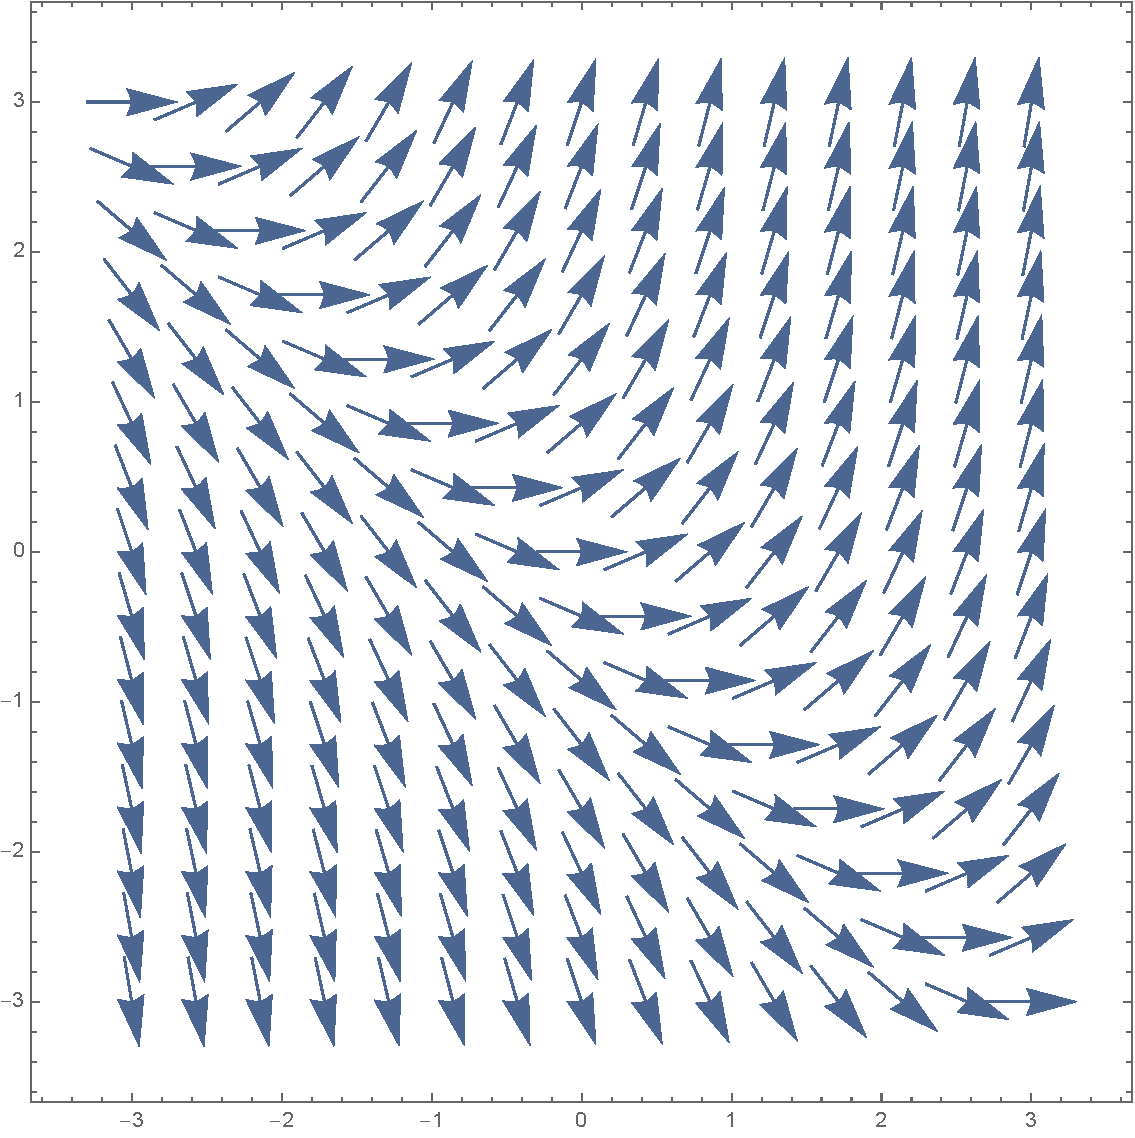
\includegraphics[width=0.45\textwidth]{./images/ch7/dfxy-1.pdf}&
			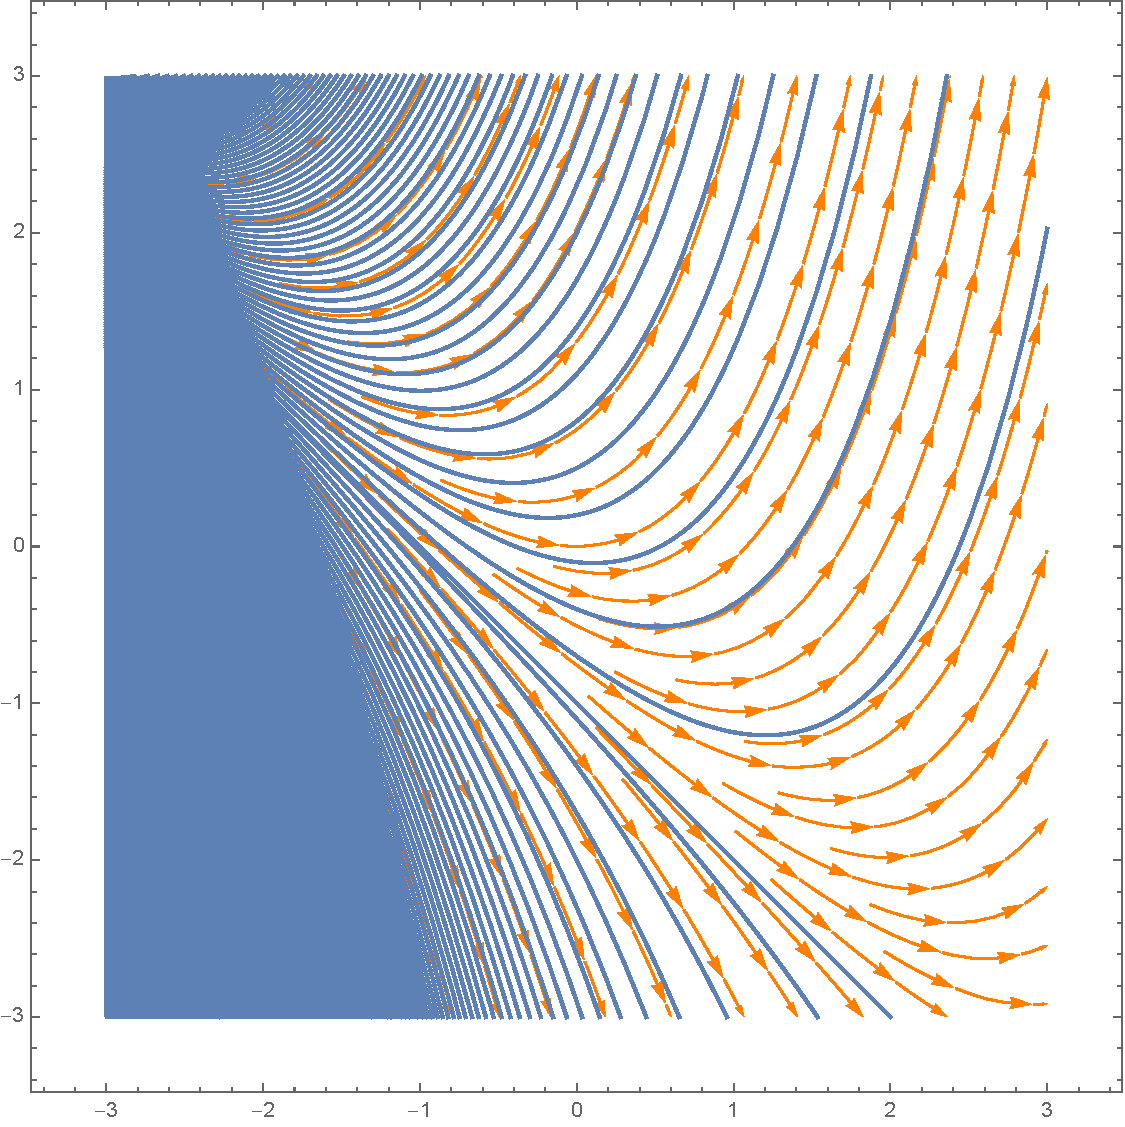
\includegraphics[width=0.45\textwidth]{./images/ch7/dfxy-4.pdf}\\
		\end{tabular}
	\end{center}
	
	同样的作法可以应用于三维的一阶微分方程组,例如著名的Lorenz方程,该方程是对
	天气预报模型的一个极简化版本,形如:
	$$
		\left\{\begin{array}{l}
			x'_t=\sigma(y-x)\\
			y'_t=x(\rho-z)-y\\
			z'_t=xy-\beta z
		\end{array}\right.
	$$
	其中$x,y,z$分别表示温度、风速和湿度。其线素场和一个特定的轨线如图:
	\begin{center}
		\begin{tabular}{cc}
			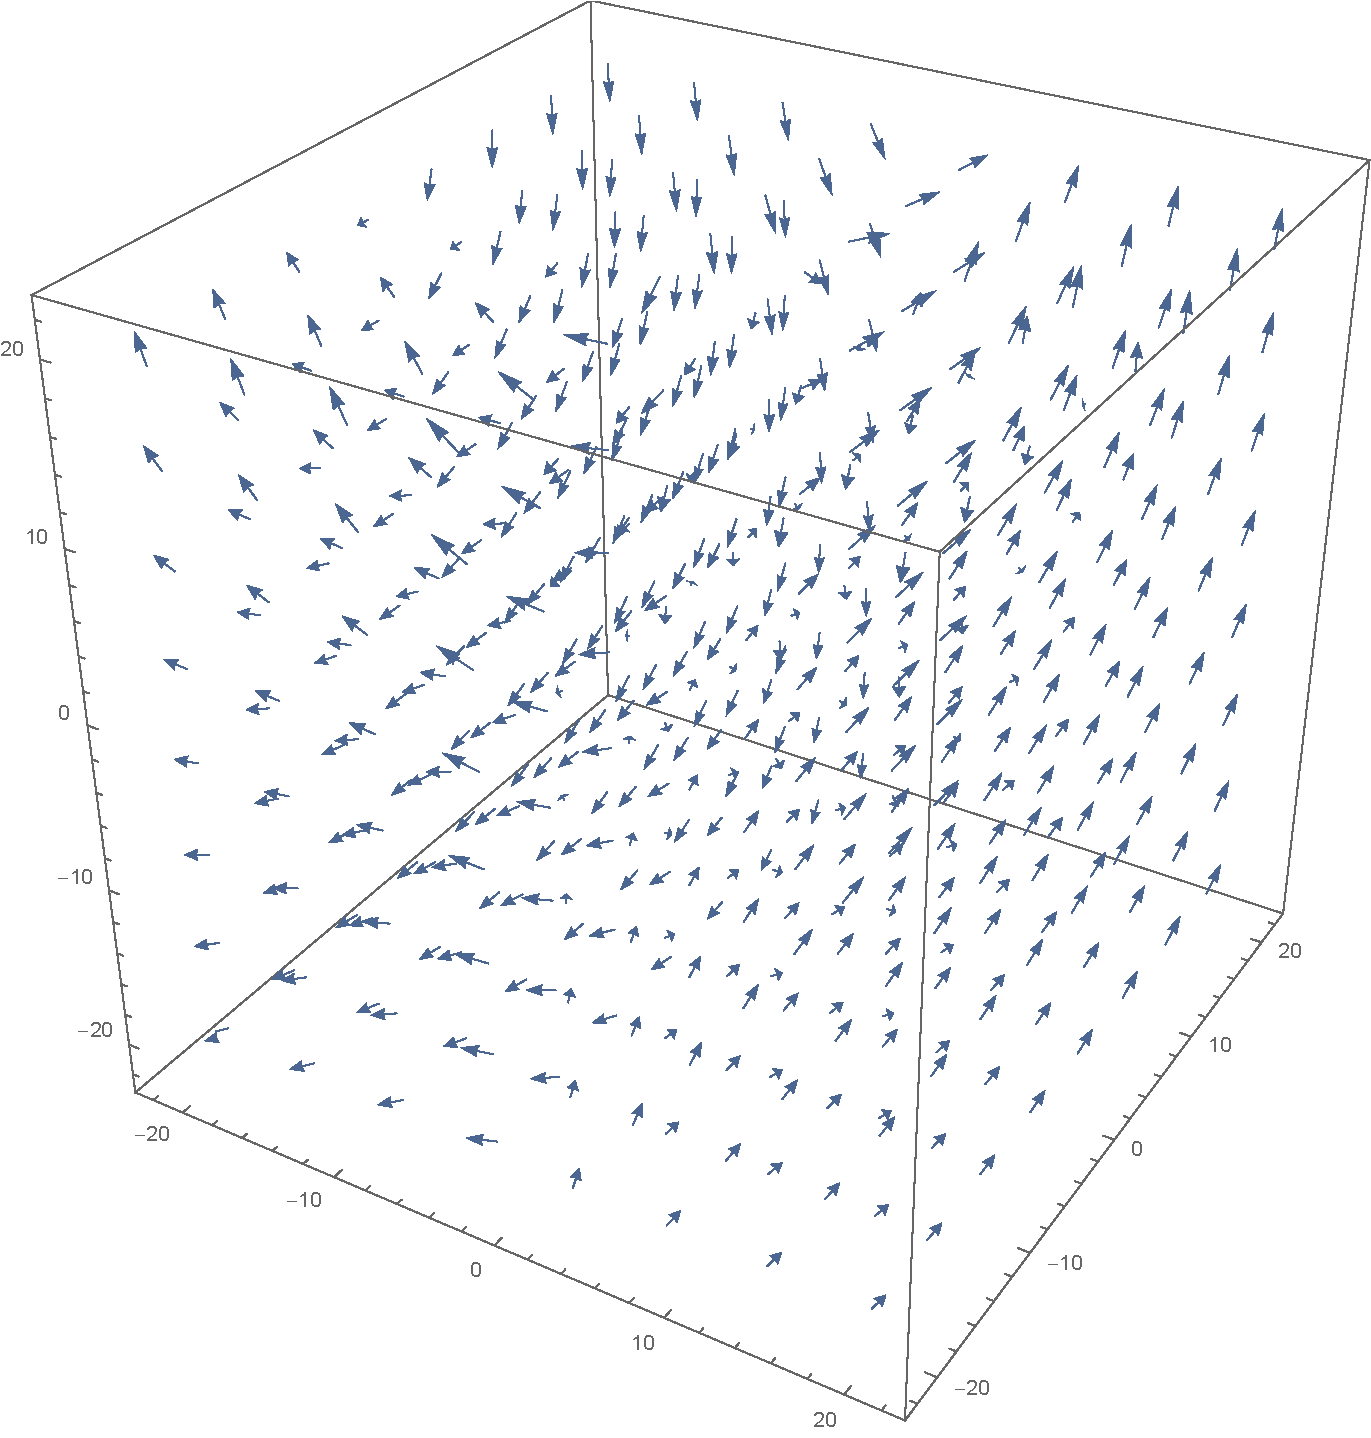
\includegraphics[width=0.45\textwidth]{./images/ch7/lorenzDF.pdf}&
			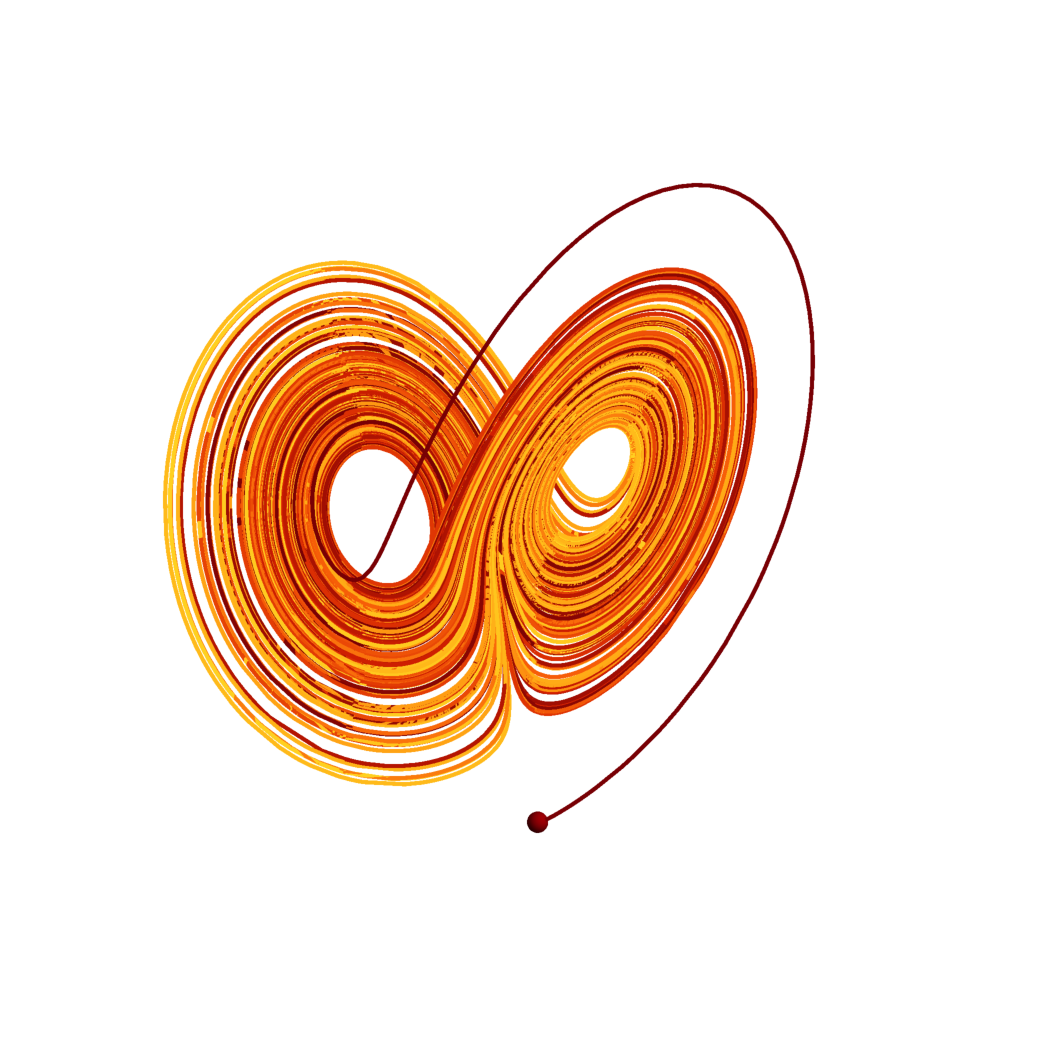
\includegraphics[width=0.45\textwidth]{./images/ch7/LorenzAtractor.pdf}\\
		\end{tabular}
	\end{center}
	图中的轨线展示的是著名的{\kaishu Lorenz吸引子},正是对它的研究
	引出了后来广为人知的	{\kaishu 蝴蝶效应}和{\kaishu 混沌现象}。
\end{shaded}

\begin{ext}
	{\bf 课后作业}
	
	\begin{enumerate}
	  \item 求解下列微分方程:
	  \begin{enumerate}[(1)]
	    \item $xy'-y+\sqrt{x^2-y^2}=0,(x>0)$
	    \item $y'=(x+y)^2$
	    \item $x\ln x\d y+(y-\ln x)\d x=0,(x>0)$ 
	    \item $3y'+y=(1-x)y^4$
	  \end{enumerate}
% 	  \item 求下列微分方程初值问题的解
% 	  \begin{enumerate}[(1)]
% 	    \item $y'+\df yx=\df{\sin x}x$,其中$y(\pi)=1$
% 	    \item $y'=\df xy+\df yx$,其中$y(1)=2$
% 	  \end{enumerate}
	  \item 某湖泊的水量为$V$,每年排入湖内的污水和净水量均为$V/6$,且湖内的总水量不变。
	  已知1999年底湖内的污染物含量为$5m_0$。为了治理污染,从2000初开始,限定排入
	  湖中的污水中污染物浓度不得超过$m_0/V$。问至少需要经过多少年,
	  湖内的污染物含量能够降至$m_0$以下?(注:假设湖水中的污染物浓度是均匀分布的。)
% 	  [提示]:$$m'=\df{m_0}6-\df m3,\quad m=\df{m_0}2(1+9e^{-t/3})$$
% 	  $t=6\ln3$年后,达到要求。
	  \item 已知$f(0)=0,f(1)=1$,且当$x\in(0,1)$时,$f''(x)<0$。任取曲线
	  $y=f(x)$上一点$(x,f(x)),\;(x\in(0,1))$,该点与原点的连线与曲线所围图形
	  面积为$x^2$,求$f(x)$。
% 	  \item 设以质量为$m$的质点作直线运动。从速度等于零的时刻起,有一个与其运动方向
% 	  一致、大小与时间成正比(比例系数为$a$)的力作用于它,与此同时地面对其的阻力
% 	  大小与其速度成正比(比例系数为$b$),求该质点的位移关于时间的函数。
	  \item 某学生将乘积的导数公式错误地记作$(fg)'=f'g'$,然而在一次求导时居然
	  得到了正确的结果。目前知道他使用的$f(x)=e^{x^2}\,(x>1/2)$,
	  问他用到的$g(x)$可能是什么?
% 	  $$\left(e^{x^2}g\right)'=\left(e^{x^2}\right)'g'$$
% 	  从而$(2x-1)g'=2xg$,解得$g=Ce^x\sqrt{|2x-1|}$
% 	  \item 
	\end{enumerate}
\end{ext}

{\bf 课堂讨论:}求解下列微分方程

% \hspace{-1ex}{\bf 【上下颠倒】}
\begin{enumerate}[(1)]
  \setlength{\itemindent}{1cm}
  \item $y'=\df{1}{2x-y^2}$ \dotfill{“上下颠倒”},$x=\df12y(y+1)+\df14+Ce^{2y}$
  \item $y'=\df{x}{x^2-y^2}$\dotfill{“上下颠倒”化为Bernoulli方程}\\
%   {\bf 【齐次方程】}
  \item $xy'=\sqrt{x^2-y^2}+y$ \dotfill{齐次方程},$y=x\sin(\ln|x|+C)$
  \item $y'=\df{3x^2+y^2-6x+3}{2xy-2y}$
  \dotfill{消去低次项变齐次方程},$3(x-1)^2-y^2=C(x-1)$\\
%   {\bf 【其他变量替换】}
  \item $xy'+y=2\sqrt{xy}$\dotfill{ 令$u=xy$},$\sqrt{xy}=x+C$
  \item $xy'+y=y(\ln x+\ln y) $ \dotfill{令$z=\ln x, w=\ln y$或$z=xy$},$xy=Ce^x$
  \item $xy'\ln x+y=ax(\ln x+1)$\dotfill{ 一阶线性方程},$y=\df12\ln x+\df C{\ln x}+1$
  \item $y'=\df{y}{2(\ln y-x)}$\dotfill{ “颠倒”,令$z=\ln y$},$y^2[1-2(\ln y-x)]=C$
  \item $y'+x=\sqrt{x^2+y}$\dotfill{ 令$z=\sqrt{x^2+y}-x$},
  $x^2+y=(x+C)(2\sqrt{x^2+y}-x)$\\
%   {\bf 【Bernouli方程】}
  \item $y'-\df{y}{x}=\df{2x}{3y^2}$ \dotfill{Bernouli方程},$y^3=Cx^3-2x^2$
  \item $2x\ln x\d y+y(y^2\ln x-1)\d x=0$\dotfill 令$z=\ln x,\df1{y^2}=\df12\ln
  x+\df C{\ln x}$\\
%   {\bf 【降阶计算】}
%   \item $y^{(4)}+y''=0$\dotfill{ 令$p=y''$}
\end{enumerate}

\section{可降阶的二阶微分方程}

高阶微分方程的求解显然需要通过多次积分,通过一步步地降低其阶数来实现。

本节以二阶微分方程
$$y''=f(x,y,y')$$
为例,介绍特定情况下一些可能的降阶方法。

\subsection{$y''=f(x,y')$型微分方程}

\begin{thx}
	{\bf 求解形如$y''=f(x,y')$的二阶微分方程:}令$y'=p(x)$,则$y''_{xx}=p'_x$,从而
	将原方程化为关于$p$和$x$的微分方程
	$$\df{\d p}{\d x}=f(x,p).$$
	由该方程解出$p(x)$,在进一步求解$y'=p(x)$即可。
\end{thx}

{\bf 例:}$xy''-y'=0$\hfill $y=\df12C_1x^2+C_2,\;(C_1,C_2\in\mathbb{R})$

利用类似的方法可以求解下面这样的高阶微分方程:

\begin{thx}
	{\bf 求解形如$y^{(n)}=f(x,y^{(n-1)})$的微分方程:}令$y^{(n-1)}=p(x)$,
	将原方程化为关于$p$和$x$的微分方程
	$$\df{\d p}{\d x}=f(x,p).$$
	由该方程解出$p(x)$,在进一步求解$y^{(n-1)}=p(x)$即可。
\end{thx}

{\bf 例:}证明:曲率为常数的平面曲线必为圆或直线。

[证]:设方程为
$$\df{|y''|}{{[1+(y')^2]^{\frac32}}}=K,\quad (K>0),$$
显然方程可以改写为
$$y''=K_1[1+(y')^2]^{\frac32},\quad (K_1\in\mbb{R}).$$
令$p(x)=y$,方程化为
$$p'=K_1[1+(y')^2]^{\frac32},$$
分离变量解之可得
$$p=\df{K_1x+C}{\sqrt{1-(K_1x+C)^2}},\quad (C\in\mbb{R}),$$
也即
$$y'=\df{K_1x+C}{\sqrt{1-(K_1x+C)^2}},$$
对其两边积分,可解得
$$y=-\df{\sqrt{1-(K_1x+C)^2}}{K_1}+C_2,\quad(C,C_2\in\mbb{R}),$$
也即
$$(x-C_1)^2+(y-C_2)^2=\df1{K_1^2},\quad (C_1,C_2\in\mbb{R}).$$

又若$K=0$,方程即为$y''=0$,其通解为$y=C_1x+C_2,\;(C_1,C_2\in\mbb{R})$。

综上可见,曲率为常数的平面曲线必为圆或直线。\fin

\subsection{$y''=f(y,y')$型微分方程}

\begin{thx}
	{\bf 求解形如$y''=f(y,y')$的二阶微分方程:}令$y'=p(y)$,则
	$$y''_{xx}=\df{\d p(y)}{\d x}=p'_y(y)p(y),$$
	从而将原方程化为关于$p$和$y$的微分方程
	$$\df{\d p}{\d y}=\df{f(y,p)}{p}.$$
	由该方程解出$p(y)$,在进一步求解$y'=p(y)$即可。
\end{thx}

{\bf 例:}$yy''+(y')^2=0$

利用类似的方法可以求解下面这样的高阶微分方程:

\begin{thx}
	{\bf 求解形如$y^{(n)}=f(y^{(n-2)},y^{(n-1)})$的微分方程:}令
	$z=y^{(n-2)}$,则方程化为
	$$z''=f(z,z'),$$
	在利用以上的解法解出$z(x)$,在求解$y^{(n-2)}=z(x)$即可。
\end{thx}

{\bf 例:}$y'y'''=3(y'')^2$

{\bf 思考:}
\begin{enumerate}[(1)]
  \setlength{\itemindent}{1cm}
  \item 总结归纳一下截止目前我们都可以求解哪些不低于二阶的微分方程?\\
  $y''=f(x),\;y''=f(x,y'),\;y''=f(y,y'), \;y''=f(y'),\;y'''=f(y',y''),\ldots$
  \item 可以推广以上的方法求解如下的微分方程吗?
  $$y''=f(x,y),\quad y^{(n)}=f(y,y^{(n-1)})$$
\end{enumerate}

{\bf 例:}证明:曲率为常数的平面曲线必为圆或直线。

[证]:设曲线方程为$y=y(x)$,曲率为$K\geq0$。由曲率的定义
$$\df{|y''|}{[1+(y')^2]^{3/2}}=K,$$
也即
$$y''=[1+(y')^2]^{3/2}K_1,\quad(K_1\in\mathbb{R}).$$

令$p(y)=y'$,则以上方程化为
$$pp'=K_1(1+p^2)^{3/2},$$
分离变量可解得
$$-\df1{\sqrt{1+p^2}}=K_1(y-C_1),\quad(C_1\in\mathbb{R})$$

若$K\ne 0$,记$R=1/K$,由上式可得
$$y'=\pm\df{\sqrt{R^2-(y-C_1)^2}}{y-C_1}.$$
进一步两边积分,可得
$$-\sqrt{R^2-(y-C_1)^2}=\pm(x-C_2),\quad(C_2\in\mathbb{R})$$
也即
$$(x-C_2)^2+(y-C_1)^2=R^2.$$

若$K=0$,则有$y''=0$,此时对应曲线方程为$y=C_1x+C_2,\;(C_1,C_2\in\mathbb{R})$.
\fin

\begin{shaded}

{\bf Einstein的宇宙膨胀模型}

假定宇宙是一个球体(半径$R(t)$),$t$表示时间,则
$$R''=-\df{GM_0}{R^2}$$
其中$G$为宇宙引力常数,$M_0$为宇宙质量。通过分析该方程可以得到关于宇宙膨胀的一些有趣的知识。

方程两端乘以$R'$可得
$$R''R'=-\df{GM_0}{R^2}R'$$
也即
$$[(R')^2]'=2GM_0\left(\df1R\right)'$$
积分可得
$$(R')^2=\df{2GM_0}R+C$$
其中$C$是和宇宙膨胀初始速度有关的常数。

下面利用上式($R'$和$R$之间的关系)确定宇宙半径是如何随时间变化的。

(1)$C>0$,此时
$$R'=\pm\sqrt{\df{2GM_0}R+C},$$
观测表明当前宇宙是膨胀的,故$R'>0$。由此可见,随着$R$越来越大,其膨胀的速度将越来越小,最终趋于
常数$\sqrt C$

(2)$-\df{2GM_0}R<C<0$,记$C=-K$,则
$$R'=\pm\sqrt{\df{2GM_0}R-K},$$
假定在某个时刻$t_0$宇宙是膨胀的,则$R'=\sqrt{\df{2GM_0}R-K}$,并且此时$\df{2GM_0}R>K$,
从而可知,当宇宙半径增加至$\df{2GM_0}R=K$时,宇宙将停止膨胀。此后,如果在某个时刻,有某种因素
引起宇宙收缩,则$R$满足
$$R'=-\sqrt{\df{2GM_0}R-K},$$
当$R$越来越小时,$\sqrt{\df{2GM_0}R-K}$越来越大,最终趋于正无穷。在此过程中,宇宙收缩的速度将
越来越快,最终发生“大坍缩”。

(3)$C=0$。假定在某个时刻宇宙是膨胀的,则
$$R'=\sqrt{\df{2GM_0}R},$$
解之可得
$$R^{\frac32}=\df32\sqrt{2GM_0}t+C_1$$
称为“平直宇宙模型”(flat universe model)

{\bf 注:}以上模型仅仅是当时科学界的一种看法,近年来,科学界又对宇宙膨胀提出了一些新的解释,比如
暗能量解释等。

\end{shaded}

\begin{ext}
	{\bf 课后作业}
	
	求解下列初值问题
	\begin{enumerate}
	  \item 求解下列初值问题
	  \begin{enumerate}[(1)]
	    \item $xy''=y',y(0)=1,y'(1)=0$
	    \item $y''+(y')^2=1,y(0)=y'(0)=1$
	    \item $y''-y=0,y(0)=0,y'(0)=1$
	  \end{enumerate}
	  \item 已知曲线$y=y(x)$光滑、严格单调递增,且经过点$(0,1)$。
	  记其上任一点$P(x,y)$处的切线与$x$轴的交点为$Q$,以$PQ$为斜边,
	  $x$轴为一条直角边的直角三角形的面积为$S_1$。对应于区间$[0,x]$的
	  曲线段与$x$轴之间的曲边梯形面积为$S_2$。已知$2S_1-S_2=1$,求
	  曲线方程。
	\end{enumerate}
\end{ext}

\section{二阶线性微分方程}

\subsection{二阶线性微分方程解的结构}

\begin{thx}
	{\bf 二阶线性微分方程解的结构:}考虑二阶齐次线性微分方程
	$$y''+p(x)y'+q(x)y=0\eqno{(1)}$$
	和二阶非齐次线性微分方程
	$$y''+p(x)y'+q(x)y=f(x)\eqno{(2)}$$
	\begin{enumerate}
	  \item 若$y_1,y_2$为(1)的解,则对任意常数$C_1,C_2$,
	  线性组合$y=C_1y_1+C_2y_2$仍为方程(1)的解;
	  \item 若以上$y_1,y_2${\kaishu 线性无关(比值不恒为常数)},
	  则以上线性组合即构成了方程(1)的通解;
	  \item 若$Y$为方程(1)的通解,$y*$为方程(2)的一个特解,则
	  $$y=Y+y*$$
	  即为方程(2)的通解。
	\end{enumerate}
\end{thx}

{\bf 例:}求以$x$和$e^x$为特解的二阶齐次线性微分方程。

[提示]:通解$C_1x+C_2e^x$,方程$(x-1)y''-xy'+y=0$。

{\bf 例:}已知微分方程$(2)$的三个解:$y_1=x,y_2=e^x,y_3=e^{2x}$,
求其满足初始条件$y(0)=1,y'(0)=3$的特解。

[提示]:(2)的任意两个特解只差必为(1)的一个特解。

\begin{thx}
	{\bf 叠加原理:}若$y_i(i=1,2,\ldots,m)$分别为方程
	$$y''+p(x)y'+g(x)y=f_i(x),\;i=1,2,\ldots,m$$
	的解,则$\sum\limits_{i=1}^my_i$为
	$$y''+p(x)y'+g(x)y=\sum\limits_{i=1}^mf_i(x)$$
	的解。
\end{thx}

{\bf 注:}显然,以上关于线性微分方程解的结构定理和叠加原理对于
高阶的线性微分方程仍然成立。

% \subsection{(部分)二阶线性微分方程的解法}

\subsection{降阶法求二阶其次线性微分方程的特解}

已知$y_1(x)$为齐次方程$y''+p(x)y'+q(x)y=0$的一个特解$y_1$,
能否/如何求得另一个与之线性无关的特解$y_2$?

\begin{thx}
	{\bf Liouville公式:}设$y_2=uy_1$,其中$u=u(x)$待定。则
	$$u{(y''_1+py'_1+qy_1)}+u'(2y'_1+py_1)+y_1u''=0,$$ 
	即$u'(2y'_1+py_1)+y_1u''=0$, 由此可解得
	$${u(x)=\dint\df{e^{-\int p(x)dx}}{y_1^2}dx}$$	
\end{thx}

对于这个公式,理解其思想比记住其结果更加重要。

{\bf 思考:}形如$y=uy_1$的变换的好处是什么?这样假设
需要满足什么特殊的条件吗?能够推广到更高阶的情形吗?

答:好处就是:{\b 将方程中函数的最低阶项系数化为$0$,使之成为可降阶的}。
这样的假设不需要任何前提条件(如果非要说有,那就是$y_1$不恒为零)。
对于更高阶的齐次线性方程,该变化同样有效!

{\bf 例:}已知$y=e^x$为方程
$$y''+\df{x}{1-x}y'-\df{1}{1-x}y=0$$
的解,求该方程的通解。\hfill $y=C_1x+C_2e^x$

{\bf 注:}给定一个二阶齐次线性微分方程,要使用Liouville公式存在一个前提:
已知该方程的一个特解$y_1$!有些情况下,可以根据方程系数的特点猜测出$y_1$:

\begin{thx}
	{\bf 通过观察得到方程$y''+p(x)y'+q(x)y=0$的一个特解:}
	
	\begin{itemize}
	  \item 若$1+p(x)+q(x)\equiv0$,则$y_1=e^x$为该方程的解
	  \item 若$1-p(x)+q(x)\equiv0$,则$y_1=e^{-x}$为该方程的解
	  \item 若$\lambda^2+\lambda p(x)+q(x)\equiv0$,则
	  $y_1=e^{\lambda x}$为该方程的解
	  \item 若$q(x)\equiv0$,则$y_1=C$为该方程的解($C$为任意常数)
	\end{itemize}
\end{thx}

事实上,有时对二阶非齐次的线性微分方程和一些高阶的方程,也可以采用类似的
“猜测”方法,例如:
\begin{itemize}
  \item 若$f(x)$恒为(非零)常数,则$y_1=\df{f(x)}{p(x)}$为方程
  $y''+p(x)y'+q(x)y=f(x)$的解;
  \item 若$1+p_1(x)+p_2(x)+p_3(x)\equiv0$,则$y_1=e^x$为方程
  $y'''+p_1(x)y''+p_2(x)y'+p_3(x)y=0$的解。
\end{itemize}

{\bf 例:}$xy''-y'-(x-1)y=0$
$$y_1=e^x,\;y=C_1e^x+C_2(2x+1)e^{-x}$$

\subsection{二阶常系数齐次线性微分方程的通解}

$$y''+py'+qy=0\;(p,q\in\mathbb{R}\mbox{为常数})$$

{\bf 特征方程(根)法:}设$y=e^{rx}$为方程的解,则
$$e^{rx}(r^2+pr+q)=0$$ 
即:$r^2+pr+q=0$ 。显然,若$r$为该{\bf 特征方程}的根,则
$y=e^{rx}$为原方程的解。

\begin{thx}
	{\bf 二阶常系数线性微分方程的通解:}
	记$\Delta=p^2-4q$, 则:
	\begin{center}
		\begin{tabular}{c|c|c|c}
			\hline
			{$\Delta$} & {$r$} & {特解} & {通解} \\ \hline 
			$\Delta>0$ & \begin{tabular}{cc}相异实根 \\ $r_1,r_2$\end{tabular} &
			$\begin{array}{ll}y_1=e^{r_1x}\\ y_2=e^{r_2x}\end{array}$ &
			{$C_1e^{r_1x}+C_2e^{r_2x}$}\\ \hline 
			$\Delta=0$ & 二重实根$r$ &
			$\begin{array}{ll}y_1=e^{rx}\\ y_2=xe^{rx}\end{array}$ &
			{$(C_1+xC_2)e^{rx}$}\\ \hline 
			$\Delta<0$ & \begin{tabular}{cc}共轭复根\\ $\alpha\pm i\beta$\end{tabular} &
			$\begin{array}{ll}y_1=e^{\alpha x}\cos\beta x\\ y_2=e^{\alpha
			x}\sin\beta x\end{array}$ & 
			{$\begin{array}{ll}e^{\alpha x}(C_1\cos\beta x +C_2\sin\beta
			x)\end{array}$}\\ \hline
		\end{tabular}
	\end{center}
\end{thx}

注:$\Delta=0$时,$y_1=e^{rx}$,由Liouville公式
$$y_2=y_1\dint\df{e^{\int p\d x}}{y_1^2}\d x
=e^{rx}\dint e^{-(p+2r)x}\d x=e^{rx}\dint\d x=xe^{rx}$$

{\bf 例:}
\begin{enumerate}[(1)]
  \setlength{\itemindent}{1cm}
  \item $y''-y'-2y=0$
  \item $\df{\d^2s}{\d t^2}+2\df{\d s}{\d t}+s=0$
  \item $y''-2y'+5y=0$
\end{enumerate}

\begin{shaded}
	{\bf $n$阶常系数齐次线性微分方程}
	$$y^{(n)}+p_1y^{(n-1)}+p_2y^{(n-2)}+\ldots+p_{n-1}y'+p_ny=0.$$
	记{\it 微分算子}$\mathrm{D}=\df{\d}{\d x}$,相应地
	$$\df{\d y}{\d x}=\mathrm{D}y,\quad \df{\d^n y}{\d x^n}=\mathrm{D}^ny,$$
	以上方程可写为
	$$(\mathrm{D}^n+p_1\mathrm{D}^{n-1}+\ldots+p_{n-1}\mathrm{D}
	+p_n)y=0.$$
	记
	$$L(\mathrm{D})=\mathrm{D}^n+p_1\mathrm{D}^{n-1}+\ldots+p_{n-1}\mathrm{D}
	+p_n$$
	为{\it 微分算子$L(\mathrm{D})$的$n$次多项式},则以上方程可进一步写为
	$$L(\mathrm{D})y=0.$$
	
	令$y=e^{rx}$,则$\mathrm{D}e^{rx}=re^{rx},\;\mathrm{D}^2e^{rx}=r^2e^{rx},
	\;\mathrm{D}^ne^{rx}=r^ne^{rx}$,故
	$$L(\mathrm{D})e^{rx}=L(r)e^{rx},$$
	由此可知如果$r$是$n$次代数方程$L(r)=0$的一个根,则$y=e^{rx}$必为前述
	$n$阶常系数齐次线性微分方程的一个解。

	{\bf 用常数变易法求二阶非齐次线性微分方程的特解}
	
	\begin{tcolorbox}
		{\bf 求二阶非齐次线性微分方程特解的常数变易法:}
		设$y_1,y_2$是对应二阶齐次线性微分方程的线性无关的解,令	
		$$
		\left\{\begin{array}{l}
		y_1C'_1+y_2C'_2=0\\
		y_1'C_1'+y'_2C'_2=f(x)
		\end{array}\right.
		$$
		解出$C_1(x)$和$C_2(x)$,则$y^*=C_1(x)y_1+C_2(x)y_2$为非齐次方程的一个特解。
	\end{tcolorbox}
	
	考虑
	$$y''+py'+qy=f(x)$$
	特征方程
	$$r^2+pr+q=0$$
	根据其根为实数或复数分别考虑如下:
	
	(1)若$r\in\mathbb{R}$,则$y=Ce^{rx}$为对应齐次方程的解,从而设特解
	$y=C(x)e^{rx}$,于是
	$$C''+(2r+p)C'=e^{-rx}f(x)$$
	$$C(x)=\dint\left[e^{-(2r+p)x}\dint e^{(r+p)x}f(x)\d x\right]\d x$$
	
	{\bf 例:}$y''+y'-2y=\sin x$
	
	设$y=C(x)e^x$,则
	$$C''+3C'=e^{-x}\sin x$$
	解得
	$$C(x)=-\df1{10}(3\sin x+\cos x)e^{-x}+C_1e^{-3x}+C_2$$
	
	{\bf 例:}$y''+4y'+4y=e^x$
	
	通解$y=\df19e^x+C_1xe^{-2x}+C_2e^{-2x}$
	
	(2)若$r=\alpha+i\beta\in\mathbb{C}$,则$y=Ce^{\alpha x}\sin\beta x$
	为齐次方程的解,从而设特解$y=C(x)e^{\alpha x}\sin\beta x$,类似地可得
	$$C(x)=\dint\left(\df{e^{-(p+2\alpha)x}\dint f(x)
	e^{(p+\alpha)x}\sin\beta x\d x}{\sin^2\beta x}\right)\d x$$
	
	{\bf 例:}$y''+y=\df1{\cos x}$
	
	$$y=\sin x\dint\df{\dint\tan x\d x}{\sin^2 x}\d x
	=\sin x(\ln|\cos x|+C_1\cos x+(x+C_2)\sin x)$$
	
	{\bf 思考:}以上方法能否推广到非常系数的情形?

	{\bf 神奇的常数变易法}
	
	所谓常数变易法,就是将齐次线性微分方程中的任意常数$C$“变易”为待定的函数$C(x)$,
	带入对应的非齐次线性微分方程,通过解出$C(x)$达到求解非齐次方程的目的。
	
	{\bf 问题1:}对一阶线性微分方程来说,常数变易法的具体过程如下:
	
	已知相对应的一阶齐次和非齐次线性
	微分方程
	$$y'+p(x)y=0\eqno{(1)},$$
	$$y'+p(x)y=f(x)\eqno{(2)},$$
	其中$f(x)$不恒为零。
	
	方程(1)通过分离变量,可求得其通解为$y=C\exp\left(-\int p(x)\d x\right)$,
	其中$C\in\mathbb{R}$为任意常数。为了求解方程(2),我们假设
	$$y=C(x)\exp\left(-\int p(x)\d x\right)$$
	为其解,其中$C(x)$为待定的函数。将其带回方程(2),化简后可得
	$$C'(x)\exp\left(-\int p(x)\d x\right)=f(x),\eqno{(3)}$$
	由此可以解得$C(x)=\int f(x)\exp\left(\int p(x)\d x\right)\d x+C_1$,
	其中$C_1\in\mathbb{R}$为任意常数。由此可知方程(2)的通解
	$$y=\left\{\int f(x)\exp\left(\int p(x)\d x\right)\d x+C_1\right\}
	\exp\left(-\int p(x)\d x\right),\quad (C_1\in\mathbb{R}).$$
	
	从形式上看,常数变易法的关键似乎是常数的“变易”,然而仔细分析可以发现,
	“变易”不过是其外在的形式,真正发挥作用的应该是如下的过程:{\it 利用齐次方程
	的一个特解$y_1$,构造非齐次方程的一个特解$y_2=u(x)y_1$,变换后使后者
	转化成一个可以降阶求解的微分方程,进而达到逐次降阶求解的目的。}其实质和
	推导Liouville公式所使用的方法是一致的。
	
	{\bf 问题2:}降阶求解二阶线性微分方程(Liouville公式)。
	
	已知二阶齐次线性微分方程
	$$y''+p_1(x)y'+p_2(x)y=0\eqno{(4)}$$
	的一个非平凡解$y_1$,可以设$y_2=u(x)y_1$为该方程的另一个解
	(需要说明是,只要$y_1$不恒为零,这样假设总是合理,或者说可以做到的)。
	将$y_2$带入方程(4),整理后可得
	$$y_1u''+(2y'_1+p_1y_1)u'=0\eqno{(5)}$$
	该方程可以通过变换$w=u'$,转化为一阶微分方程
	$$y_1w'+(2y'_1+p_1y_1)w=0,$$
	求解该方程,再经过多次的积分还原,最终可以求得$y_2$。
	
	分析以上的推导过程,不难发现,令$y_2=u(x)y_1$发挥了关键性的作用,
	通过这样的转换,{\it 新的方程(5)中不再含有未知函数($u(x)$)的非导数项,从而
	使之可以通过变换$w=u'$实现降阶},并最终完成求解。
	
	回过头来再看问题1,其中所谓常数“变易”的实质和问题2中的令$y_2=u(x)y_1$
	并没有本质的不同。事实上,$y_1=\exp\left(-\int p(x)\d x\right)$
	为方程(1)的特解,通过将$C$改为$C(x)$来构造(2)的解,就相当于令$y_2=C(x)y_1$
	为(2)的解,这样做的效果就是使转换后的方程中不再含有未知函数($C(x)$)的
	非导数项,从而使之能够通过积分直接求解,并最终达到了求解非齐次方程的目的。
	
	至此我们发现,求解一阶非齐次线性微分方程的常数变易法的降阶求解二阶线性微分
	方程的Liouville公式原来具有内在的一致性,就是在已知齐次方程的一个特解$y_1$
	的前提下,利用$y_2=u(x)y_1$的形式来构造待求的其他解。因为这样的构造形式
	可以消去方程中含有未知函数的项,从而使得方程可进一步降阶或者直接进行求解。
	
	了解了该方法的特性,我们不难推广得到如下的一些结论:
	
	{\bf 问题3:}利用$y_2=u(x)y_1$构造二阶非齐次线性微分方程的特解。
	
	已知二阶齐次线性微分方程(4)的一个非平凡解$y_1$,
	设$y_2=u(x)y_1$为对应的二阶非齐次线性微分方程
	$$y''+p_1(x)y'+p_2(x)y=f(x)\eqno{(6)}$$
	的解。
	
	将$y_2$带入方程(6),整理后可得
	$$y_1u''+(2y'_1+p_1y_1)u'=f(x)\eqno{(7)}$$
	再令$w=u'$,该方程可以进一步化为
	$$y_1w'+(2y'_1+p_1y_1)w=f(x),$$
	这是一个一阶非齐次线性微分方程,是可解的。
	
	至此我们可以对求解二阶非齐次线性微分方程的方法稍加总结:
	
	[第一步] 寻找对应齐次线性微分方程的一个非平凡特解$y_1$;
	
	[第二步] 利用Liouville公式,解出齐次线性微分方程的另一个
	线性无关的特解$y_2$;
	
	[第三步] 设$y^*=u(x)y_1$为非齐次线性微分方程的一个解,
	带入方程化解出$y^*$(参考例3的过程)
	
	[第四步] 根据线性微分方程解的结构,非齐次线性微分方程的通解为
	$$Y=C_1y_1+C_2y_2+y^*,\quad (C_1,C_2\in\mathbb{R}).$$
	
	这一方法能够完整实现的前提是[第一步]找到对应齐次线性微分方程的一个非
	平凡特解,后续过程则主要集中于具体的积分计算。
	
	根据全国研究生入学考试数学一考试大纲的要求,目前国内高等数学教材中,
	都包含了利用特征方程法求解二阶常系数齐次线性微分以及进一步利用
	待定系数法求解对应的二阶常系数非齐次线性微分的方法(参见同济大学教材)。
	这一方法的优点是,应用简便(不需要要到积分),计算量相对较小,并且从考试命题的角度
	来说,也便于构造各种不同形式的考题。但其一个明显的缺点就是,能够求解
	的方程类型过于狭窄,只能求解自由项$f(x)$为特定形式(例如:
	$P(x)e^{\lambda x}$和$(P(x)\sin{\lambda x}+P(x)\cos{\lambda x})
	e^{\mu x}$)的常系数微分方程。此外,对待定系数法的构造思想的理解一直
	也是教学中的一个巨大的难点。
	
	相对而言,我们以上总结的方法,虽然在计算量和推导过程上看,都更为复杂和繁琐,
	但其使用的思想确实特别简单和易于理解的。(讲义的下一小节中,我们结合教材的例6,展示了
	两种方法在计算过程上的比较)。
	
	最后,在一些高等数学的教材上(例如我们前面提到过的),还介绍了求解二阶非齐次线性微分方程的
	常数变易法。
	
	{\bf 问题4:}求解二阶非齐次线性微分方程的常数变易法。

	已知$y_1,y_2$是二阶齐次线性微分方程(4)的线性无关的解,
	可设$y^*=C_1(x)y_1+C_2(x)y_2$为其对应非齐次方程(5)的解,则
	$$(y^*)'=C'_1y_1+C_1y'_1+C'_2y_2+C_2y'_2,$$
	由于我们只需要求方程(5)的一个特解,
	{\it 为了消去转化后方程中关于未知函数$C_1(x)$和$C_2(x)$的项},可以令
	$$C'_1y_1+C'_2y_2=0,\eqno{(8)}$$
	于是进一步有
	$$(y^*)''=C'_1y'_1+C_1y''_1+C'_2y'_2+C_2y''_2,$$
	带入方程(5)化简后可得
	$$y_1'C_1'+y'_2C'_2=f(x),\eqno{(9)}$$
	联立方程(8)(9),可以解出$C'_1(x)$和$C'_2(x)$,然后积分得到$C_1(x)$和$C_2(x)$,
	并最终得到$y^*$。
	
	该方法之所以被称为常数变易法,直接的原因也是因为其形式上相当于将齐次方程(4)
	通解$C_1y_1+C_2y_2$中的常数$C_1$和$C_2$“变易”为未知函数$C_1(x)$和$C_2(x)$,
	以此来构造和求解对应非齐次方程的解。但我们应该看到,其实质和利用$y_2=u(x)y_2$
	的方法来构造新的解并无本质的不同,因为其最终的效果都是消去了新方程中关于
	未知函数$C_1(x)$和$C_2(x)$的项,从而到了一种便于求解的结构。

	这一方法经过推广,可以应用于利用$n$阶齐次线性微分方程的通解,求解对应
	$n$阶非齐次线性微分方程的通解。
	
	{\bf 问题5:}由$n$阶齐次线性微分方程的通解求对应非齐次方程的通解。
	
	已知$n$阶齐次线性微分方程
	$$y^{(n)}+p_1(x)y^{(n-1)}+p_2(x)y^{(n-2)}+\ldots+p_{n-1}(x)y'
	+p_n(x)y=0,\eqno{(10)}$$
	的通解$\sum\limits_{k=1}^nC_ky_k,\;(C_1,C_2,\ldots,C_n\in\mathbb{R})$,
	可以假设对应非齐次线性微分方程
	$$y^{(n)}+p_1(x)y^{(n-1)}+p_2(x)y^{(n-2)}+\ldots+p_{n-1}(x)y'
	+p_n(x)y=f(x)\eqno{(11)}$$
	的特解
	$$y^*=\sum\limits_{k=1}^nC_k(x)y_k.$$
	于是
	$$(y^*)'=\sum\limits_{k=1}^nC'_ky_k+\sum\limits_{k=1}^nC_ky'_k,$$
	与前述方法类似,令
	$$\sum\limits_{k=1}^nC'_ky_k=0,\eqno{(12)}$$
	进而有
	$$(y^*)''=\sum\limits_{k=1}^nC'_ky'_k+\sum\limits_{k=1}^nC_ky''_k,$$
	继续令
	$$\sum\limits_{k=1}^nC'_ky'_k=0,\eqno{(13)}$$
	进而又有
	$$(y^*)'''=\sum\limits_{k=1}^nC'_ky''_k+\sum\limits_{k=1}^nC_ky'''_k,$$
	类似地假设新的条件,并进行推导化简。最后,假设
	$$\sum\limits_{k=1}^nC'_ky^{(n-2)}_k=0,\eqno{(11+n-1)}$$
	从而方程(11)化为
	$$\sum\limits_{k=1}^nC'_ky^{(n-1)}_k=f(x).\eqno{(11+n)}$$
	
	联立方程(12)(13)\ldots(11$+n$),也即
	$$\left[\begin{array}{cccc}
	y_1 & y_2 & \ldots & y_n\\
	y'_1 & y'_2 & \ldots & y'_n\\
	\ldots & \ldots & \ldots &\ldots\\
	y^{(n-1)}_1 & y^{(n-1)}_2 & \ldots & y^{(n-1)}_n
	\end{array}
	\right]
	\left[\begin{array}{c}
	C'_1 \\ C'_2 \\ \ldots \\ C'_n 
	\end{array}\right]
	=\left[\begin{array}{c}
	0 \\ 0 \\ \ldots \\ f(x)
	\end{array}\right]$$
	由此解出$C'_k(x),(k=1,2,\ldots,n)$,再积分求得$C_k(x),(k=1,2,\ldots,n)$,
	即可得到$y^*$。最终利用线性微分方程解的结构定理,即得方程(11)的通解。
	
	
	讨论:我们前面描述的求解二阶非齐次线性微分方程一般方法,在一定条件下是可以推广
	到更高阶的线性微分方程的。事实上,如果能够已知某$n$阶齐次线性微分方程一个非平凡解$y_1$,
	总可以令$y_2=u(x)y_1$为其另一个解,然后使方程化为可降阶为$n-1$解方程的形式。
	接下来,再递归地使用以上思路(前提是对每一次降阶的方程都能够找到某个非平凡的特解),
	最终达到逐步降阶逐步求解原方程的目的。
	
	[TBD]这里需要一个例子。
\end{shaded}

\subsection{用待定系数法求部分二阶常系数非齐次线性方程的特解}

关键是求得该方程的一个特解!

{\bf 情形一:}{\b$f(x)=e^{\lambda x}P_m(x)$,其中$P_m(x)$为$m$阶多项式,
$\lambda$为常数

{\bf 解法:}设方程的特解为
$$y^*=x^ke^{\lambda x}(a_0+a_1x+\ldots+a_mx^m),$$
其中$k=0,1,2$分别对应与$\lambda$不是特征方程的根、
是特征方程的重根和单根的情况}

% \newpage

{\bf 例:}$y''-2y'-3y=e^{3x}(1+x^2)$

[解一]:
设原方程有特解$y^*=e^{3x}x(a_0+a_1x+a_2x^2)$,代回原方程利用待定系数法解得
$a_0=\df9{32},a_1=-\df1{16},a_2=\df1{12}$,
故该方程的通解为
$$y=C_1e^{-x}+C_2e^{3x}+e^{3x}x\left(\df9{32}-\df{x}{16}+\df1{12}x^2\right)$$

\begin{shaded}
	[解二]:	(用常数变易法求解)
	显然,该方程对应的齐次方程的通解为$C_1e^{-x}+C_2e^{3x},(C_1,C_2\in\mathbb{R})$。
	设$y^*=C(x)e^{3x}$为原方程的一个特解,带入方程化简可得
	$$C''+4C'=1+x^2\eqno{(E1)},$$
	令$C'=w(x)$,方程(E1)化为$w'+4w=1+x^2$,利用一阶线性微分方程的常数变易法可解得
	$C'=w=\df9{32}-\df18x+\df14x^2+C_3$,不妨令$C_3=0$,进而可得
	$$C(x)=\df9{32}x-\df1{16}x^2+\df1{12}x^3+C_4.$$
	不妨令$C_4=0$,从而可得原方程的通解为
	$$y=C_1e^{-x}+C_2e^{3x}+e^{3x}x\left(\df9{32}-\df{x}{16}+\df1{12}x^2\right),
	(C_1,C_2\in\mathbb{R}).$$
		
	{\bf 注:}{\it 以上两种解法都存在很大的计算量,但是相对而言,使用常数变易法解题的思路更为
	直观清晰,便于随时检查验算阶段性的计算结果,推荐使用。}
\end{shaded}

% \newpage

{\bf 例:}$y''-6y'+9y=e^{3x}+9$
$$y=C_1e^{3x}+C_2xe^3x+\df12x^2e^{3x}+1$$

{\bf 情形二:}{\b $f(x)=e^{\alpha x}[P_m(x)\cos\beta x+P_l(x)\sin\beta x]$,
其中$P_m(x),P_l(x)$分别为$m,l$阶多项式,$\beta\ne 0$

{\bf 解法:}设方程的特解为
$$y^*=x^ke^{\alpha x}[R^{(1)}_n(x)\cos\beta x+R^{(2)}_n(x)\sin\beta x]$$ 
其中:$n=\max\{m,l\}$,$R^{(1)}_n(x),R^{(2)}_n(x)$均为次数不超过$n$的多项式;
若$\alpha+i\beta$是特征方程的根,取$k=1$,否则取$k=0$。} 

{\bf 例:}$y''+4y=\cos 2x$

设$y^*=x(A\cos2x+B\sin2x)$,通解
$$y=C_1\cos2x+C_2\sin2x+\df x4\sin2x$$

{\bf 例:}一根挂在钉子上的链条,最初两端距离钉子分别为$8$m和$12$m,如不计钉子
对链条产生的摩擦力,求链条从钉子上完全滑落所需的时间。

设$x$为较长一端端点据钉子的距离
$$\left\{\begin{array}{l}
	x''-\df g{10}x=-g\\
	x(0)=12\\
	x'(0)=0
\end{array}\right.$$

\subsection{Eular方程}

$${\b x^2y''+pxy'+qy=f(x)\quad(p,q\in\mathbb{R}\mbox{为常数})}$$

{\bf 解:}令{\b$x=e^t$},则
$$y'_x=\df1xy'_t,\;y''_{xx}=\df1{x^2}(y''_{tt}-y'_t),$$
即
$$x^2y''_{xx}=y''_{tt}-y'_t,\;xy'_x=y'_t,$$
原方程可化为二阶常系数线性微分方程
$$y''_{tt}+(p-1)y'_t+qy=f(e^t)$$

{\bf 例:}$x^2y''+xy'-y=0$

$$y''_tt-y=0,\quad y=\df{C_1}x+C_2x$$

{\bf 思考:}以上解法对于我们求解高阶Euler方程有何启示?\hfill{\bf 辅导书(下)-P230}

事实上,$x^3y'''_{xxx}=\df1{x^3}(y'''_{ttt}-3y''_{tt}+2y'_t)$,故
{\b 以上的方法可以推广到三阶},特别是$f(x)=0$的情形,例如:
$$x^3y'''+px^2y''+qxy'+ry=0$$

那么,还可以进一步推广吗?请课后自行推理!

\begin{shaded}
	{\bf $n$阶Euler方程}
	$$x^ny^{(n)}+p_1x^{n-1}y^{(n-1)}+\ldots+p_{n-1}xy'
	+p_ny=f(x).$$
	
	令$x=e^t$,则
	\begin{align*}
		\df{\d y}{\d x}&=\df1x\df{\d y}{\d t},\\
		\df{\d^2 y}{\d x^2}&=\df1{x^2}\left(\df{\d^2 y}{\d t^2}
		-\df{\d y}{\d t}\right),\\
		\df{\d^3 y}{\d x^3}&=\df1{x^3}\left(\df{\d^3 y}{\d t^3}
		-3\df{\d^2 y}{\d t^2}+2\df{\d y}{\d t}\right).
	\end{align*}
	记$\mathrm{D}=\df{\d}{\d t}$,则以上结果可写为
	\begin{align*}
		xy'&=\mathrm{D}y,\\
		x^2y''&=\mathrm{D}(\mathrm{D}-1)y,\\
		x^3y'''&=\mathrm{D}(\mathrm{D}-1)(\mathrm{D}-2)y.
	\end{align*}
	一般地,有
	$$x^ky^{(k)}=\mathrm{D}(\mathrm{D}-1)\ldots(\mathrm{D}-k+1)y.$$
	
	{\bf 例:}解方程$x^3y'''+x^2y''-4xy'=3x^2$.
	
	[解]:令$x=e^t$,方程可化为
	$$\mathrm{D}(\mathrm{D}-1)(\mathrm{D}-2)y+\mathrm{D}(\mathrm{D}-1)y
	-4\mathrm{D}y=3e^{2t},$$
	也即
	$$(\mathrm{D}^3-2\mathrm{D}^2-3\mathrm{D})y=3e^{2t}.$$
	\ldots\ldots
	
	原方程的通解为
	$$y=C_1+\df{C_2}x+C_3x^3-\df12x^2,\quad(C_1,C_2,C_3\in\mathbb{R}).$$
\end{shaded}

\begin{ext}
	{\bf 课后作业}
	\begin{enumerate}
	  \item 求解下列微分方程
	  \begin{enumerate}[(1)]
	    \item $y''-y=e^x+\cos x$
	    \item $y^{(4)}+y''=1$
	  \end{enumerate}
	  \item 求级数$\sumn[0]\df{x^{2n}}{(2n)!}$的和函数。
	  \item 设$\varphi'(x)=e^x+\sqrt x\dint_0^{\sqrt x}\varphi(\sqrt x u)\d u,$
	  $\varphi(0)=0$,求$\varphi(x)$。
	  \item 设$y(x)$在$\mathbb{R}$上具有二阶连续导数,$y'\ne 0$,$x=x(y)$
	  为其反函数。
	    \begin{enumerate}[(1)]
	      \item 试将$x=x(y)$所满足的微分方程
	      $$\df{\d^2x}{\d y^2}+(y+\sin x)\left(\df{\d x}{\d y}\right)^3=0$$
	      变换为$y=y(x)$所满足的微分方程;%\hfill$y''-y=-\sin x$
	      \item 求变换后的微分方程满足初始条件$y(0)=0$和$y'(0)=1.5$的解。
	    \end{enumerate}
	    \item 设以质量为$m$的质点作直线运动。从速度等于零的时刻起,有一个与其运动方向
		一致、大小与时间成正比(比例系数为$a$)的力作用于它,与此同时地面对其的阻力
		大小与其速度成正比(比例系数为$b$),求该质点的位移函数$S(t)$(设初始位移$S(0)=0$)。
% 	    \item 
	  \end{enumerate}
% 	  设特解$y^*=A\cos x+B\sin x$,解得$A=0,B=1/2$,故通解
% 	  $$y=C_1e^x+C_2e^{-x}+\df12\sin x,$$
% 	  利用初值条件,得所求特解
% 	  $$y=e^x-e^{-x}+\df12\sin x$$
\end{ext}

\section{小结}

微分方程经常被认为是高等数学中最难掌握的内容,究其原因无外有二:一是方程类型众多,
套路不一,且方程的形式稍加变化,即导致所学习的“套路”失效;二是求解过程中需要进行
大量的积分计算,不会积分常常成为很多同学的“拦路虎”。

学习微分方程的解法,思路上应重点把握两点:一是变换,特别是对于一阶方程,通过变换将
所给的方程化成常见的形式,是求解的关键;二是降阶,当然是对高阶方程而言,一些常见的
“套路”需要时时牢记于心。

从考试的角度,通过变换求解各种可能形式的一阶微分方程和求解二阶常系数非齐次线性微分方程,
一直都是“热点”,特别是后者结合高阶线性微分方程解的结构,可以演化出许多不同类型的题目,
具体的例子在教学辅导书上有很多。

\newpage

\section*{作业参考解答}

\begin{center}
	\bf 7.1 概念与应用
\end{center}

1.请给出如下通解对应的微分方程,并给出其满足给定初值条件的特解:
  \begin{enumerate}[(1)]
    \setlength{\itemindent}{1cm}
    \item $y=x^2+C_1x+C_2$,其中$C_1,C_2$为任意常数,$y(0)=y'(0)=1$; 
    \item $y=\df{1+Ce^t}{1-Ce^t}$,其中$C$为任意常数,$y(0)=2$;
    \item $y=(C_1+C_2x)e^x$,其中$C_1,C_2$为任意常数,$y(0)=0,y'(1)=1$。
% 	\item $y=C_1\sin x+C_2\cos x+e^x$,其中$C_1,C_2$为任意常数,$y(0)=0,y'(\pi)=0$。
  \end{enumerate}

[解]:(1)原方程两边对$x$连续两次求导,可得
$$y'=2x+C_1,\quad y''=2,$$
即为所求方程。

将$y(0)=y'(0)=1$分别带入通解和上述第一个方程可得$C_1=C_2=1$,故
所求特解为$y=x^2+x+1$。

(2)原方程可化为
$$C=\df{y-1}{y+1}e^{-t},$$
两边对$t$求导,可得
$$0=\df{2y'-y^2+1}{(y+1)^2}e^{-t},$$
从而可得
$$2y'-y^2+1=0,\quad(y\ne-1),$$
即为所求方程。

将$y(0)=2$带入通解可得$C=\frac13$,从而所求特解为
$y=\df{3+e^t}{3-e^t}$。


(3)原方程可化为
$$ye^{-x}=C_1+C_2x,$$
两边对$x$连续两次求导,可得
$$(y'-y)e^{-x}=C_2,\quad
(y''-2y'+y)e^{-x}=0.$$
因为$e^{-x}\ne0$,故所求方程即为
$$y''-2y'+y=0.$$

又将$y(0)=0,y'(1)=1$带入通解和前述第一个方程中,可得
$C_1=0,C_2=\frac1{2e}$,从而所求特解为$y=\frac12xe^{x-1}$。
\fin

\bs

2.设河边点$O$的正对岸为点$A$,河宽$h$,两岸平行,水流速度恒定为$a$。
一只鸭子从点$A$游向点$O$,游动过程中其始终朝向$O$点。已知鸭子在
静水中的游速为$b(b>a)$,以$O$为原点,水流方向为$x$轴,垂直于水流
过河的方向为$y$轴,试给出鸭子的运动轨迹所满足的微分方程初值问题。

[解]:如图,
\begin{center}
	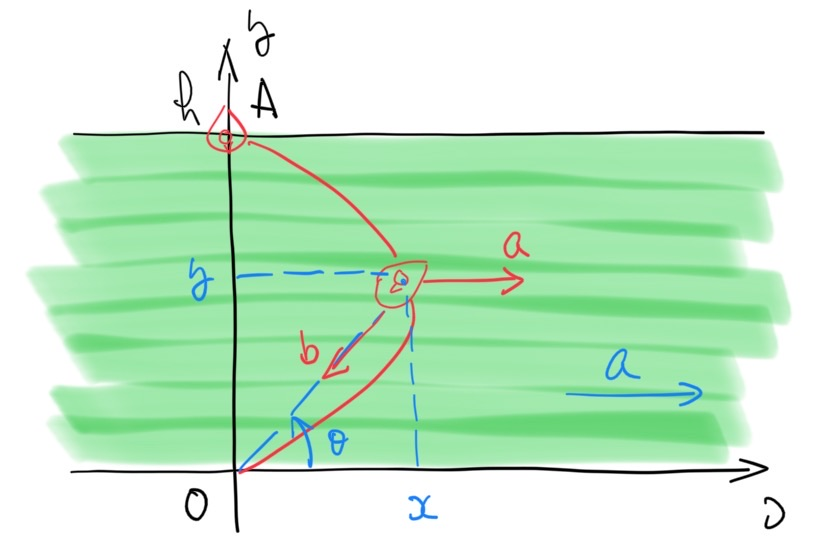
\includegraphics[width=0.5\textwidth]{./images/ch7/duck.jpg}
\end{center}
在鸭子运动轨迹上任一点$(x,y)$处,其运动满足
$$x'_t=a-b\cos\theta,\quad y'_t=-b\sin\theta,$$
其中
$$\sin\theta=\df{y}{\sqrt{x^2+y^2}},\quad
\cos\theta=\df{x}{\sqrt{x^2+y^2}},$$
故
$$y'_x=\df{y'_t}{x'_t}=\df{-by}{a\sqrt{x^2+y^2}-bx},$$
显然$y(0)=h$,故所求初值问题为
$$
	\left\{\begin{array}{l}
		y'=\df{-by}{a\sqrt{x^2+y^2}-bx},\\
		y(0)=h.
	\end{array}\right.
$$
\fin

\bs

\begin{center}
	\bf 7.2 一阶微分方程的解法
\end{center}

1.求解下列微分方程:
  \begin{enumerate}[(1)]
    \setlength{\itemindent}{1cm}
    \item $xy'-y+\sqrt{x^2-y^2}=0,(x>0)$
    \item $y'=(x+y)^2$
    \item $x\ln x\d y+(y-\ln x)\d x=0$ 
    \item $3y'+y=(1-x)y^4$
  \end{enumerate}

[提示]:(1)令$z=\frac yx$,则原方程可化为
$$xz'+\sqrt{1-z^2}=0.$$
当$\sqrt{1-z^2}\ne 0$时,该方程分离变量,解得$z=\sin(-\ln x+C)$。
当$\sqrt{1-z^2}=0$时,方程有解$y=\pm x$。

综上,原方程的解为
$$y=x\sin(\ln x+C),\;(x\in\mbb{R})
\quad\mbox{或}\quad y=\pm x.$$

(2)令$z=x+y$,则原方程可化为
$$z'-1=z^2,$$
该方程分离变量,解得$z=\tan(x+C)$,进而原方程的解为
$$x+y=\tan(x+C),\;(C\in\mbb{R}).$$

(3)令$u=\ln x$,则原方程可化为
$$u\d y+(y-u)\d u=0,$$
该方程是一个齐次方程(也是一个全微分方程),可解得
$2yu-u^2=C$,故原方程的解为
$$(2y-\ln x)\ln x=C,\;(C\in\mbb{R}).$$

(4)该方程为Bernoulli方程。当$y\ne0$时,令
$z=y^{-3}$,则原方程可化为
$$-z'+z=1-x,$$
该方程为一阶非齐次线性微分方程,可解得
$z=-x+Ce^x$。显然$y=0$是方程的特解。综上原方程的解为
$$y^3(-x+Ce^x)=1,\;(C\in\mbb{R}),\;\mbox{或}\;y=0.$$
\fin

\bs

2.某湖泊的水量为$V$,每年排入湖内的污水和净水量均为$V/6$,且湖内的总水量不变。
已知1999年底湖内的污染物含量为$5m_0$。为了治理污染,从2000初开始,限定排入
湖中的污水中污染物浓度不得超过$m_0/V$。问至少需要经过多少年,
湖内的污染物含量能够降至$m_0$以下?(注:假设湖水中的污染物浓度是均匀分布的。)

[解]:设$m(t)$为自2000年起第$t$年时湖内的污染物总量,则
$$m'=\df{m_0}6-\df{m}3,$$
且$m(0)=5m_0$。解之可得
$$m=\df{m_0}2\left(1+9e^{-\frac13t}\right).$$
令$m<m_0$,可得$t>3\ln9\approx6.59$,故大约7年后,湖水中的污染物含量可以
降至$m_0$以下。\fin

3.已知$f(0)=0,f(1)=1$,且当$x\in(0,1)$时,$f''(x)<0$。任取曲线
$y=f(x)$上一点$(x,f(x)),\;(x\in(0,1))$,该点与原点的连线与曲线所围图形
面积为$x^2$,求$f(x)$。

[解]:如图,
\begin{center}
	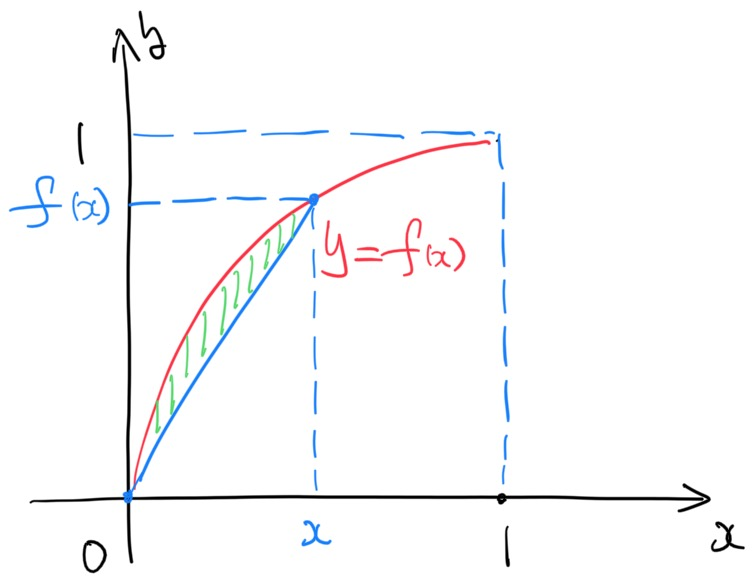
\includegraphics[width=0.45\textwidth]{./images/ch7/fxx2.jpg}
\end{center}
由已知
$$\dint_0^xf(t)\d t-\df12xf(x)=x^2,\quad x\in[0,1],$$
两边求导,整理得
$$f(x)-xf'(x)=4x.$$
该方程为一阶非齐次线性微分方程,解之得
$$f(x)=(-4\ln x+C)x,\;(C\in\mbb{R},x\in(0,1)),$$
带入$f(1)=1$,可解得$C=1$,从而所求曲线的方程为
$$f(x)=\left\{\begin{array}{ll}
	0,& x=0,\\
	(-4\ln x+1)x,& x\in(0,1].
\end{array}\right.$$
\fin

\bs

4.某学生将乘积的导数公式错误地记作$(fg)'=f'g'$,然而在一次求导时居然
得到了正确的结果。目前知道他使用的$f(x)=e^{x^2}\,(x>1/2)$,
问他用到的$g(x)$可能是什么?

[解]:由已知
$$(e^{x^2}g(x))'=(e^{x^2})'g'(x),$$
展开化简可得
$$2xg=(2x-1)g',$$
该方程分离变量,求解可得
$$g(x)=Ce^x\sqrt{2x-1},\;(x>\frac12).$$
\fin

\bs

\begin{center}
	\bf 7.3 可降阶的二阶微分方程
\end{center}

1.求解下列初值问题

(1)$xy''=y',y(0)=1,y'(1)=0$

[解]:令$p(x)=y'$,则原方程即为
$$xp'=p,$$
分离变量可解得$p=Cx,\;(C\in\mbb{R})$,也即
$$y'=Cx,$$
从而可得
$$y=C_1x^2+C_2,\quad (C_1,C_2\in\mbb{R}),$$
带入初值条件可得$C_2=1,C_1=0$,故所求方程的特解为
$$y=1.$$

\bs

(2)$y''+(y')^2=1,y(0)=y'(0)=1$

[解]:令$p(x)=y'$,则原方程即为
$$p'+p^2=1,$$
注意到$p(0)=y'(0)=1$,故必有$p=y'=1$,进而可得
$$y=x+C,$$
又$y(0)=1$,可得$C=1$,从而所求特解为
$$y=x+C.$$

\bs

(3)$y''-y=0,y(0)=0,y'(0)=1$

[解]:令$p(y)=y'$,则原方程化为
$$pp'-y=0,$$
分离变量解之可得$p=\sqrt{y^2+C_1},\;(C_1\in\mbb{R})$,也即
$$y'=\sqrt{y^2+C_1},$$
带入初值条件,可解得$C_1=1$,进而
$$y'=\sqrt{y^2+1},$$
分离变量解之可得
$$y=\df{e^{x+C_2}-e^{-(x+C_2)}}2,\quad (C_2\in\mbb{R}),$$
在此带入初值条件,可得$C_2=0$,故所求方程的特解为
$$y=\df{e^x-e^{-x}}2.$$
\fin

\bs

2.已知曲线$y=y(x)$光滑、严格单调递增,且经过点$(0,1)$。
记其上任一点$P(x,y)$处的切线与$x$轴的交点为$Q$,以$PQ$为斜边,
$x$轴为一条直角边的直角三角形的面积为$S_1$。对应于区间$[0,x]$的
曲线段与$x$轴之间的曲边梯形面积为$S_2$。已知$2S_1-S_2=1$,求
曲线方程。

[解]:如图
\begin{center}
	\resizebox{!}{7cm}{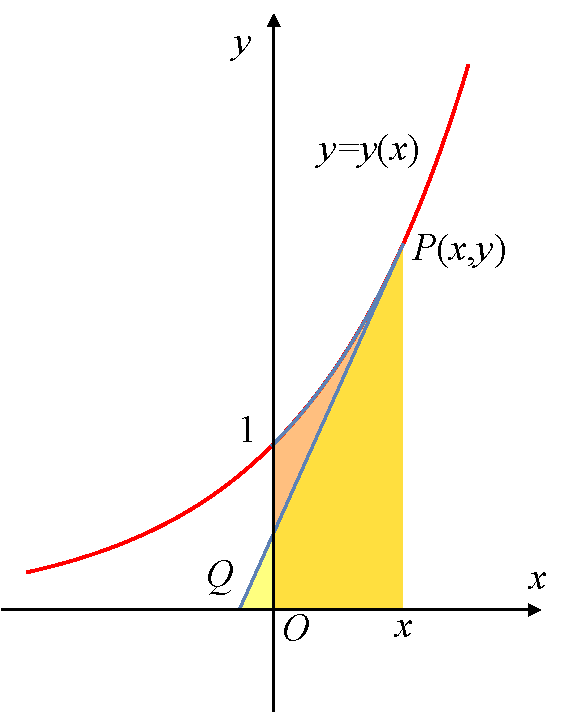
\includegraphics{./images/ch7/eX.pdf}}
\end{center}
设所求曲线为$y=y(x)$,过其上任一点$P(x,y)\;(x\geq 0)$的切线为
$$Y=y+y'(X-x),$$
与$x$轴相交于$Q(x-x/y',0)$。由于$y'>0$,故当$x\geq 0$时,恒有$y\geq 1$,故
$$S_1=\df12y\left[x-\left(x-\df{y}{y'}\right)\right]=\df{y^2}{2y'}.$$
又
$$S_2=\dint_0^xy(t)\d t,$$
由已知$2S_1-S_2=1$,也即
$$\df{y^2}{y'}-\dint_0^xy(t)\d t=1.$$

对该方程两边连求导,并取$x=0$可得
$$\left\{\begin{array}{l}
yy''=(y')^2\\
y(0)=1\\
y'(0)=1
\end{array}\right.$$
解之得$y=e^x$,即为所求。\fin

\bs

\begin{center}
	\bf 7.4 二阶线性微分方程
\end{center}

1.求解下列微分方程
  \begin{enumerate}[(1)]
    \setlength{\itemindent}{1cm}
    \item $y''-y=e^x+\cos x$
    \item $y^{(4)}+y''=1$
  \end{enumerate}

[解]:(1)该方程的特征方程为$r^2-1=0$,特征根为$r=\pm1$,
故其对应的齐次方程的通解为$y=C_1e^x+C_2e^{-x},(C_1,C_2\in\mbb{R})$。

利用叠加原理,可以设原方程的特解为
$$y^*=Axe^x+(B\cos x+C\sin x),$$
带入原方程可得
$$2Ae^x-2B\cos x-2C\sin x=e^x+\cos x,$$
从而可得$A=\frac12,B=-\frac12,C=0$。

综上,原方程的通解为
$$y=C_1e^x+C_2e^{-x}+\df12xe^x-\df12\cos x,\quad (C_1,C_2\in\mbb{R})$$

\bs

(2)令$z=y''$,则原方程可化为
$$z''+z=1,$$
求解该方程可得其通解为$z=C_1\cos x+C_2\sin x+1,(C_1,C_2\in\mbb{R})$,
也即
$$y''=C_1\cos x+C_2\sin x+1,$$
对其两边连续两次积分可得
$$y=C_3\cos x+C_4\sin x+\df12x^2+C_5x+C_6,\quad (C_3,C_4,C_5,C_6\in\mbb{R}),$$
即为原方程的通解。\fin

\bs

2.求级数$\sumn[0]\df{x^{2n}}{(2n)!}$的和函数。

[解]:该级数的收敛域为$(-\infty,+\infty)$,设其和函数为$S(x)$,则
$$S''(x)=S(x).$$
这是一个二阶常系数齐次线性微分方程,解之可得
$$S(x)=C_1e^x+C_2e^{-x},\quad(C_1,C_2\in\mbb{R}).$$
注意到$S(0)=1,S'(0)=0$,带入以上的通解,可得$C_1=C_2=\frac12$,故
$$\sumn[0]\df{x^{2n}}{(2n)!}=\df{e^x+e^{-x}}2,\quad(x\in\mbb{R}).$$
\fin

\bs

3.设$\varphi'(x)=e^x+\sqrt x\dint_0^{\sqrt x}\varphi(\sqrt x u)\d u,$
$\varphi(0)=0$,求$\varphi(x)$。

[解]:令$t=\sqrt xu$,则已知方程即为
$$\varphi'(x)=e^x+\dint_0^x\varphi(t)\d t,$$
对其两边关于$x$求导,结合已知条件,可得到初值问题
$$
	\left\{\begin{array}{l}
		\varphi''(x)-\varphi(x)=e^x,\\
		\varphi(0)=0,\\
		\varphi(0)=1.
	\end{array}\right.
$$
解之可得
$$\varphi(x)=\df14e^x-\df14e^{-x}+\df12xe^x.$$
\fin

\bs

4.设$y(x)$在$\mathbb{R}$上具有二阶连续导数,$y'\ne 0$,$x=x(y)$
  为其反函数。
    \begin{enumerate}[(1)]
      \setlength{\itemindent}{1cm}
      \item 试将$x=x(y)$所满足的微分方程
      $$\df{\d^2x}{\d y^2}+(y+\sin x)\left(\df{\d x}{\d y}\right)^3=0$$
      变换为$y=y(x)$所满足的微分方程;%\hfill$y''-y=-\sin x$
      \item 求变换后的微分方程满足初始条件$y(0)=0$和$y'(0)=1.5$的解。
    \end{enumerate}

[解]:(1)
$$\df{\d^2x}{\d y^2}=\df{\d x'}{\d y}
=\df{\d(1/y')}{\d y}=
\df{\df{\d\frac1{y'}}{\d x}}{\df{\d y}{\d x}}=-\df{y''}{(y')^3},$$
从而原方程可化为
$$y''-y=\sin x.$$
(2)以上方程对应的齐次方程的通解为$y=C_1e^x+C_2e^{-x},(C_1,C_2\in\mbb{R})$。
设该方程的特解为$y^*=A\cos x+B\sin x$,带入方程可得
$$-2A\cos x-2B\sin x=\sin x,$$
从而可得$A=0,B=-\frac12$,故该方程的通解为
$$y=C_1e^x+C_2e^{-x}-\df12\sin x,\quad (C_1,C_2\in\mbb{R}).$$
\fin

\bs

5.设以质量为$m$的质点作直线运动。从速度等于零的时刻起,有一个与其运动方向
一致、大小与时间成正比(比例系数为$a$)的力作用于它,与此同时地面对其的阻力
大小与其速度成正比(比例系数为$b$),求该质点的位移函数$S(t)$(设初始位移$S(0)=0$)

[解]:由已知
$$S''(t)=\df{at}m-\df{bS'(t)}m.$$
该方程对应的齐次方程的通解为$S(t)=C_1+C_2e^{-\frac{bt}m},(C_1,C_2\in\mbb{R})$。

设该方程的特解为$S^*(t)=(At+B)t$,带入方程可得
$$2A+\df bm(2At+B)=\df{at}m,$$
由此解得$A=\df{a}{2b},B=-\df{ma}{b^2}$。

综上原方程的通解为
$$S(t)=C_1+C_2e^{-\frac{bt}m}+\df{at^2}{2b}-\df{mat}{b^2},
\quad (C_1,C_2\in\mbb{R})$$

又$S(0)=S'(0)=0$,带入通解中可得$C_1=\frac{m^2a}{b^3},C_2=-\frac{m^2a}{b^3}$,
进而所求位移函数为
$$S(x)=\frac{m^2a}{b^3}\left(1-e^{-\frac{bt}m}\right)
+\df{at^2}{2b}-\df{mat}{b^2}.$$
\fin

% \section*{课后作业}
% \addcontentsline{toc}{section}{课后作业}
% 
% 
% {\bf 【必作题】}
% 
% \begin{itemize}
%   \setlength{\itemindent}{1cm}
%   \item 习题7.1:6,8,13
%   \item 习题7.2:3,4(2,3,5,6),6(1,2),7,8
%   \item 求解如下方程
% 	\begin{enumerate}[(1)]
% 	  \setlength{\itemindent}{1cm}
% 	  \item $y'=\df{1}{2x-y^2}$
% 	  \item $y'=\df{x}{x^2-y^2}$
% 	  \item $xy'=\sqrt{x^2-y^2}+y$
% 	  \item $y'=\df{3x^2+y^2-6x+3}{2xy-2y}$
% 	  \item $xy'+y=2\sqrt{xy}$
% 	  \item $xy'+y=y(\ln x+\ln y) $
% 	  \item $xy'\ln x+y=ax(\ln x+1)$
% 	  \item $y'=\df{y}{2(\ln y-x)}$
% 	  \item $y'+x=\sqrt{x^2+y}$
% 	  \item $y'-\df{y}{x}=\df{2x}{3y^2}$
% 	  \item $2x\ln x\d y+y(y^2\ln x-1)\d x=0$
% 	\end{enumerate}
%   \item 习题7.3:2(1,3,5),4,7(注:倒数第二行$[0,1]$改为$[0,x]$)
%   \item 习题7.4:6,12,13,14(1)
%   
% \end{itemize}
% 
% \bigskip
% 
% \hrule
% 
% \bigskip
% \bigskip
% 
% {\bf 【思考题】}
% 
% \begin{itemize}
%   \setlength{\itemindent}{1cm}
%   \item 习题7.2:12
%   \item 习题7.3:3,5
%   \item 习题7.4:8,9,11,13,15,16
% \end{itemize}

% \newpage
% 
% \section*{习题参考解答}
% \addcontentsline{toc}{section}{习题参考解答}
% 
% % {\it 注:以下题目的编号和顺序可能与作业有所不同,请留意!欢迎纠错:)}
% 
% {\bf 习题7.1}
% 
% \bigskip
% 
% 6.\;(1)$y'=\df{2y}x-1$,\quad (2)$y''=2y'-y$
% 
% \bigskip
% 
% 8.\;$y''x=4x-y'$
% 
% \bigskip
% 
% 13.
% 
% 
% 
% \bigskip
% 
% {\bf 习题7.2}
% 
% \bigskip
% 
% 3.\; (1)$y=\tan(x-1)$\quad (2)$\ln|y|+\df12y^2=\sin x+\df12$
% \quad (3)$y=\sqrt{1+2x^2}$
% 
% \quad(4)$\cos y=\df{\sqrt2}4(e^x+1)$\quad(5)$y^2-x^2=y^3$
% \quad(6)$y^2=2(\ln x+1)x^2$
% 
% \bigskip
% 
% 4.\;(2)$\df23(x+1)^{\frac72}+C(x+1)^2$\quad(3)$y=-x^2+Cx^3$
% 
% \quad(4)$y\cos x=x+C$\quad(5)$xy=-\cos x+C$\quad(6)$4xy=y^4+C$
% 
% \bigskip
% 
% 6.\;(1)$x^2+y^2+y+\df12=Ce^{2y}$\quad (2)$y(Ce^x-\sin x)=1$
% 
% \bigskip
% 
% 7.\;解:在已知等式中令$x=y=0$,可得$f(0)=1$。又对任意$x$,
% \begin{align*}
% 	f'(x)&=\lim\limits_{\Delta x\to0}\df{f(x+\Delta x)-f(x)}{\Delta x}
% 	=\lim\limits_{\Delta x\to0}\df{f(x)f(\Delta x)-f(x)f(0)}{\Delta x}\\
% 	&=f(x)\lim\limits_{\Delta x\to0}\df{f(\Delta x)-f(0)}{\Delta x}
% 	=f(x)f'(0)=2f(x)
% \end{align*}
% 求解初值问题:$f'(x)=2f(x),f(0)=1$,可得$f(x)=e^{2x}$。
% 
% \bigskip
% 
% 8.\;解:原式两边同时关于$x$求导,整理后可得
% $$\dint_0^xy(t)\d t=x^2y+\dint_0^xty(t)\d t,$$
% 再次求导可得
% $$x^2y'=-(3x-1)y,$$
% 利用分量变量法求解,可得其通解为$x^3y=Ce^{-1/x}$,即为所求。
% 
% 
% 
% 2.\;(1)$y=x^3+x+1$\quad(3)$y=2-\ln4+\ln x^2$\quad(5)$y=e^{-x}$

\visibletrue

\ifvisible

	\newpage
	
	{\bf 关于“神之课代表”所写题目的解释:}
	
	{\it 题目来源:辅导书(下)-P242-例10-18,题目及解答如图:}
	
	\begin{center}
		\resizebox{!}{7cm}{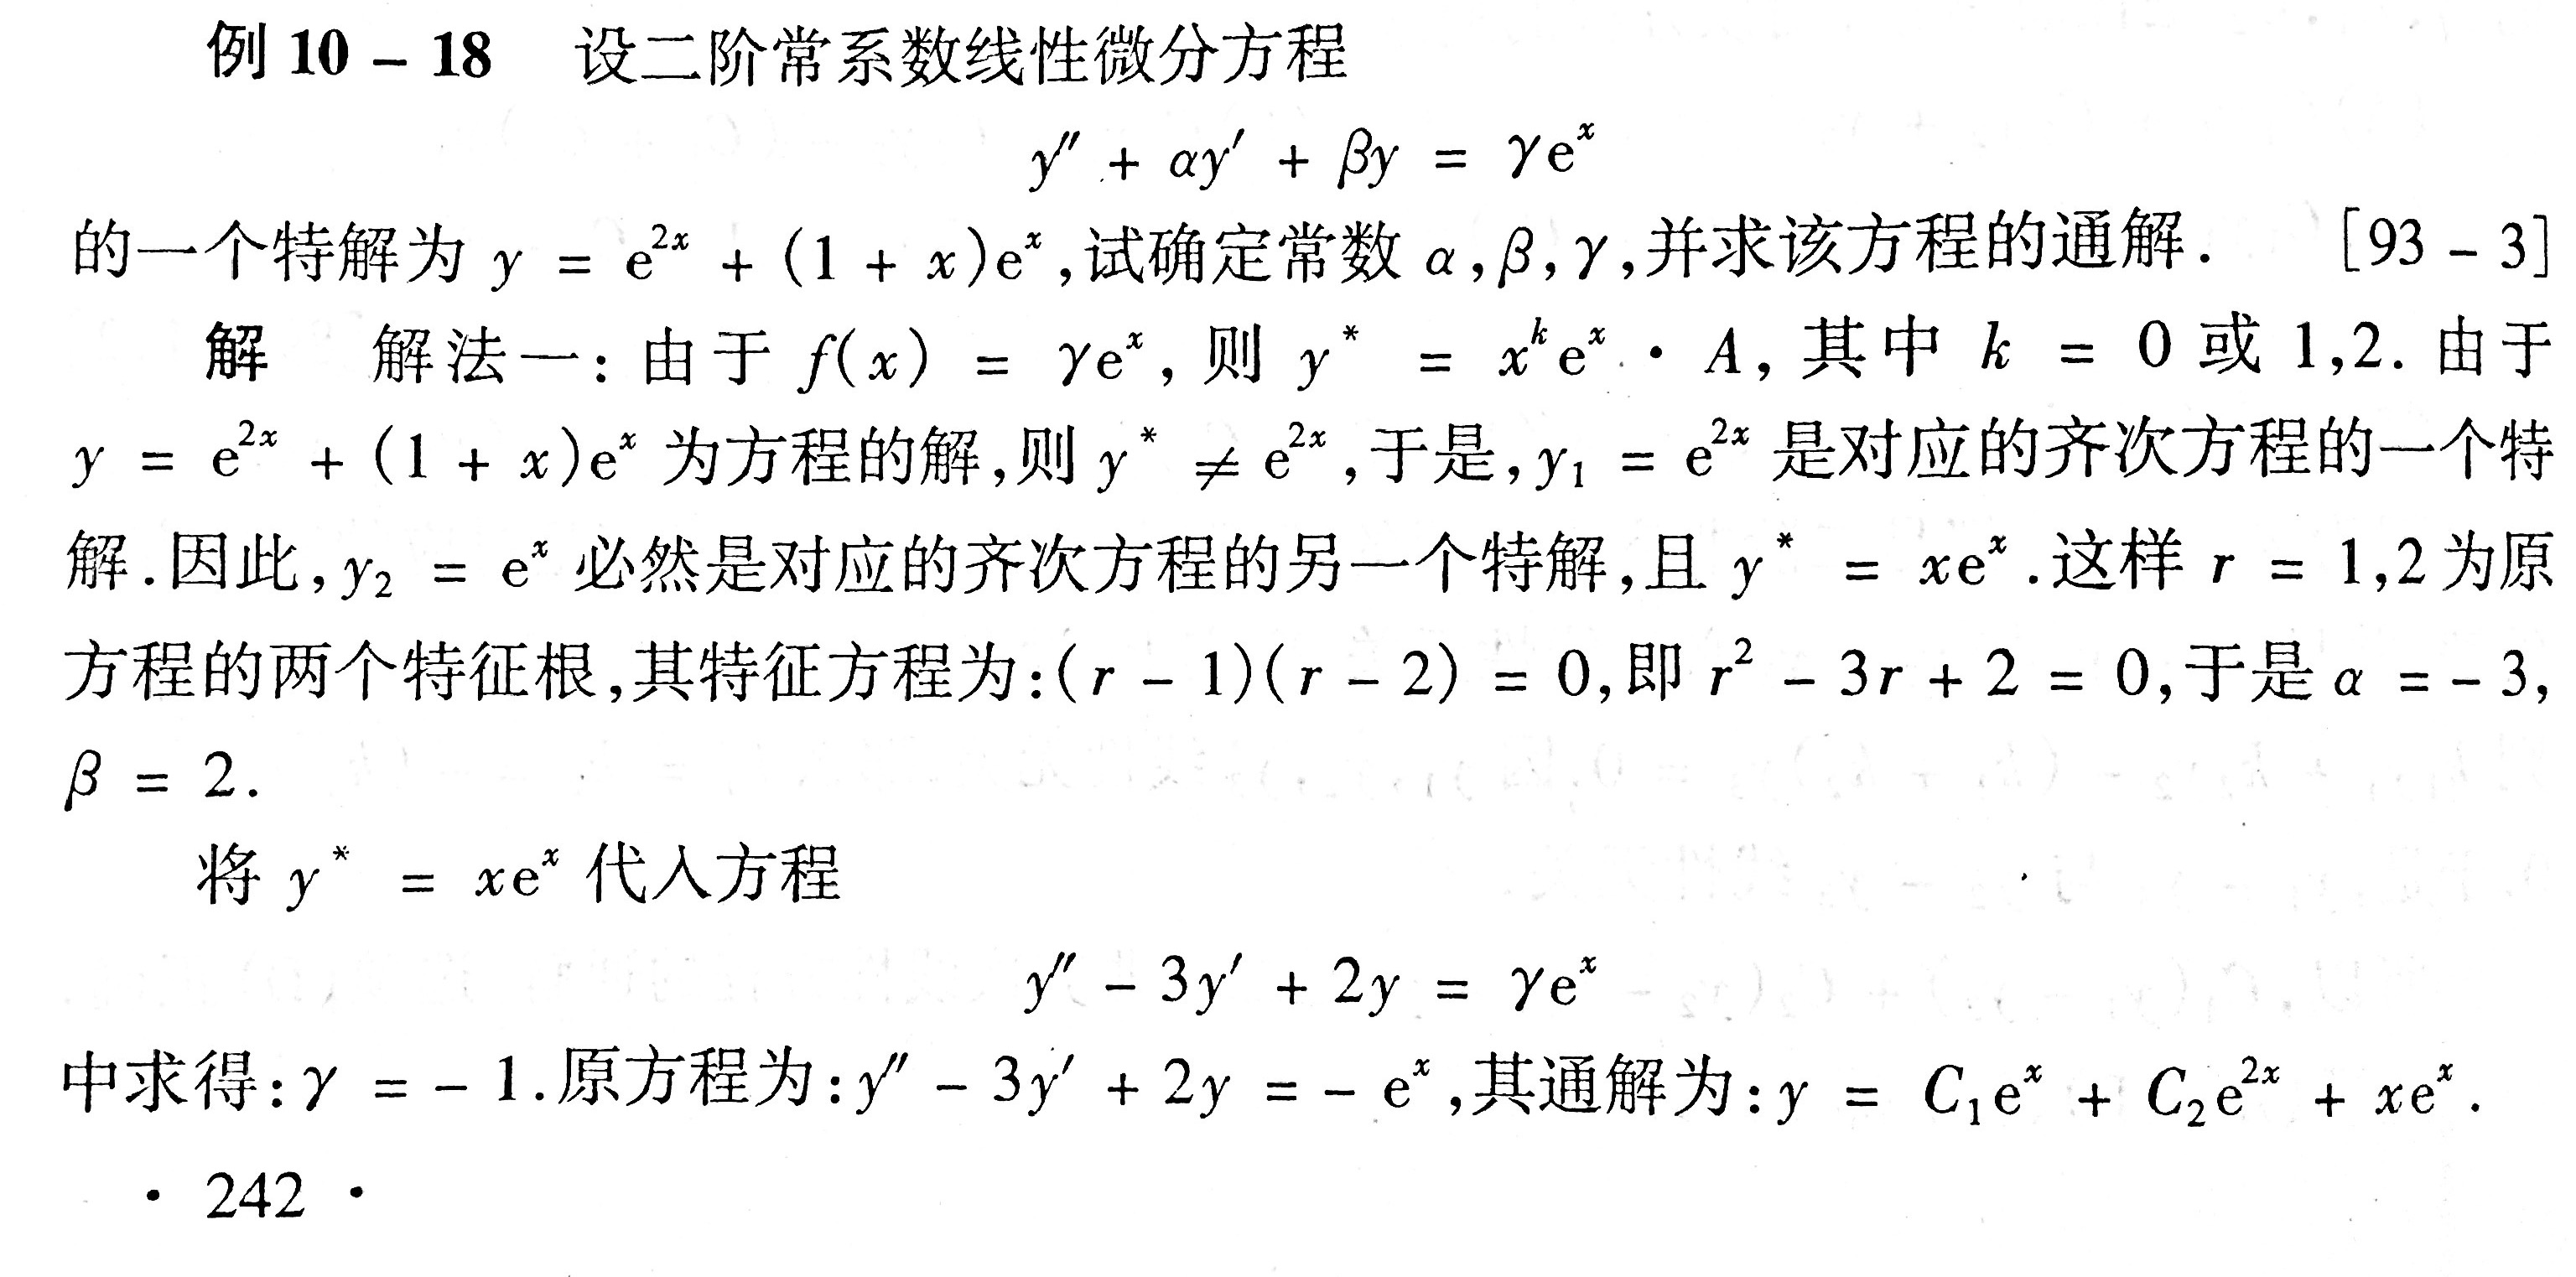
\includegraphics{./images/ch7/p242.jpg}}
	\end{center}
	
	{\it 这个解答没有问题,只是有些简略,导致不好理解。以下是我在此基础上进一步细化后的解答:}
	
	{\bf 解:}由于右端函数为$\gamma e^x$,故原方程的特解应该形如
	$$y^*=x^ke^x,$$
	其中$k$可能为$0,1,2$。
	
	根据线性微分方程解的结构定理,非齐次线性微分方程的特解可以由对应的齐次方程的多个特解与
	该非齐次方程的一个特解相加得到。以下利用该结论进行分析:
	
	注意到
	$$(e^{2x})''+\alpha(e^{2x})'+\beta e^{2x}
	=(4+2\alpha+\beta)e^{2x},$$
	故$e^{2x}$不可能是原(非齐次)方程的特解,从而只能是对应的齐次方程的特解。
	由此可知,$r=2$是方程的特征方程的根,
	
	根据上一步的结论,可知$(1+x)e^x$中必然包含了原(非齐次)方程的特解,现在的问题是要将
	这个特解的部分找出来。在此我们可以断言$(1+x)e^x$这个整体不可能就是原(非齐次)方程的特解
	(因为它不具备前述$y^*$所应有的形式),特解只能是$e^x$和$xe^x$之一。
	换言之,$e^x$和$xe^x$两者一个是原(非齐次)方程的特解,另一个是对应的齐次方程的特解。
	
	若$xe^x$是对应的齐次方程的特解。根据二阶常系数齐次线性微分方程的通解公式,只有当$r=1$
	为其特征方程的二重根时,解才会有形如$C_1e^x+C_2xe^x$的构造。而由前面的分析我们
	已知$r=2$是特征方程的一个根,故$xe^x$只能是原(非齐次)方程的特解。进而$y=e^x$
	必然是对应的齐次方程的特解。
	
	综上可知,原(非齐次)方程有特解$xe^x$,其特征方程有相异实根$r=1,r=2$。
	
	以下步骤和原解答相同,略。
	
% 	\newpage
% 	
% 	\section*{作业要求}
% 	
% 	\begin{center}
% 		(试行版,2015年春季学期)
% 	\end{center}
% 	
% 	\begin{enumerate}
% 	%   \setlength{\itemindent}{1cm}
% 	  \item 作业内容分为基本题、上交题和思考题三部分,前两部分为必作题
% 	  \item 上交与批改
% 	  \begin{itemize}
% 	    \item 作业分两部分分别上交
% 	    \item 基础题每周上交一次,由本连负责人收齐交当周轮值的同学批改
% 	    \item 上交题及思考题(选作)分三组,每周由其中一组上交,教员负责批改,
% 	    每次上交须包括前两周未交过的部分
% 	  \end{itemize}
% 	  \item 基础题批改
% 	  \begin{itemize}
% 	    \item 按照事先排定的值班顺序,确保每人本学期至少轮值一次批改其他同学的作业
% 	    \item 轮值同学批改其他同学作业后,须
% 	    \begin{itemize}
% 	      \item 根据作业正确率按百分制为其打分
% 	      \item 在作业纸上签名
% 	      \item 汇总作业情况交给本连负责人,汇总内容包括
% 	      \begin{itemize}
% 	        \item 每人的作业成绩
% 	        \item 作业中大家错误或疑问较多的题目
% 	      \end{itemize}
% 	    \end{itemize}
% 	    \item 连负责人将本连作业情况汇总后交总课代表
% 	  \end{itemize}
% 	\end{enumerate}
	
	\newpage

\section{附录}

\subsection{内容小结}

{\it\b 以下最后加*的内容不作重点掌握,了解即可。}

\begin{enumerate}[1.]
%   \setlength{\itemindent}{1cm}
  \item 基本概念
  \begin{enumerate}[(1)]
    \item 通解、特解、初值问题
    \item {\it 积分曲线、线素场、包络}*
    \item {\it 微分方程建模}*
  \end{enumerate}
  \item 一阶微分方程
  \begin{enumerate}[(1)]
    \item 可分离变量的方程\dotfill$\df{\d y}{g(y)}=f(x)\d x$,
    不要遗漏$g(y)=0$中包含的特解
    \item 一阶线性微分方程\dotfill 常数变易法,理解构造的原理
    \item 齐次方程\dotfill$z=\df yx$
    \item Bernoulli方程\dotfill$z=y^{1-n},n\ne0,1$,理解变换的原理
    \item 其他:全微分方程、导数上下颠倒,换元,积分方程
  \end{enumerate}
  \item 两类可降阶的方程(情形)
  \begin{enumerate}[(1)]
    \item $y''=f(x,y')$\dotfill令$y'=p(x)$,则$y''=p'$;可推广到$y^{(n)}=f(x,y^{(n-1)})$
    \item $y''=f(y,y')$\dotfill$y'=p(y)$,则$y''=p'p$;
    可以推广到$y^{(n)}=f(y,y^{(n-1)})$
    \item $y^{(n)}=f(y^{(n-1)},y^{(n-2)})$\dotfill$y^{(n-2)}=z$,则$z''=f(z',z)$
  \end{enumerate}
  \item 二阶线性微分方程
  \begin{enumerate}[(1)]
    \item 解的结构\dotfill 对于高阶的线性微分方程仍然成立
    \begin{itemize}
      \item 若齐次方程的有线性无关的特解$y_1,y_2$,则通解为:
      $$Y=C_1y_1+C_2y_2,\;(C_1,C_2\in\mathbb{R})$$
      \item 若非齐次方程有特解$y^*$,则通解为$Y+y^*$
      \item 叠加原理
    \end{itemize}
    \item {\it 利用$\bm{y=uy_1}$使方程化为可降阶的形式}*
    \begin{itemize}
      \item {\it 齐次方程}\dotfill Liouville公式
      \item {\it 非齐次方程}\dotfill 常数变易法的二阶(高阶)推广
    \end{itemize}
    \item 求常系数齐次线性微分方程的通解\dotfill 特征根法;可以推广到高阶的常系数线性微分方程
    \item 求特定二阶常系数非齐次线性微分方程特解的待定系数法
    \item Eular方程:\dotfill 令$x=e^t$,原方程化为常系数线性微分方程
  \end{enumerate}
\end{enumerate}

\subsection{问题讨论}

{\bf 例:}判定分析
\begin{enumerate}[(1)]
  \setlength{\itemindent}{1cm}
  \item 以下推导是否正确? 
	$$xy'=y\quad \Rightarrow\quad y=0\;\mbox{或}\;\df{\d y}{y}=\df{\d x}{x}$$
	 $$\Rightarrow\quad y=0\;\mbox{或}\;\ln |y|=\ln
	|x|+C_1\;(C_1\in\mathbb{R})$$
	 
	故方程通解为:
	$$y=Cx\;\quad (C\in\mathbb{R})$$
	 	
	{\bf 答:}正确!
  \item  已知$n$阶线性微分方程的$n$个解,能否写出这个微分方程及其通解? 
	
  {\bf 答:}不一定。 除非{这$n$个解恰为$n$阶齐次线性微分方程的线性无关的特解。} 
  \item 适当确定微分方程通解中的参数值,可以得到其任意的特解? 
	
  {\bf 答:}错!反例:$xy'=y^2$。
  \item $y_1=(x-1)^2$和$y_2=(x+1)^2$ 都是方程
	$$(x-1)^2y''-2xy'+2y=0,$$
	和
	$$2yy''-(y')^2=0$$
	的解。 但二者的线性组合
	$$y=c_1(x-1)^2+c_2(x+1)^2,\;(c_1,c_2\in\mathbb{R})$$
	 却仅能满足前一个方程, 为什么?
  
  {\bf 答:}第二个方程不是齐次线性方程!
  \item 求以$(x+C)^2+y^2=1$为通解的微分方程。
  {\bf 答:}$(y')^2=\df1{y^2}-1$。
\end{enumerate}

\subsection{方程求解}

{\bf 例:}求解如下方程

(1)$y'=\df1{2x-y^2}$

解:原方程即为
$$\df{\d x}{\d y}-2x=-y^2,$$
由一阶非齐次线性微分方程的常数变易法,解得
$$x=\df12y(y+1)+\df14+Ce^{2x},(C\in\mathbb{R})$$

(2)$y'=\df{x}{x^2-y^2}$

解:原方程即为
$$\df{\d x}{\d y}-x=-\df{y^2}x,$$
该方程为Bernoulli方程,令$z=x^2$,可得
$$z'_y-2z=-2y^2,$$
利用一阶非齐次线性微分方程的常数变易法,解得
$$x^2=z=y^2+y+\df12+Ce^{2y},(C\in\mathbb{R})$$

(3)$xy'=\sqrt{x^2-y^2}+y$

解:原方程即为
$$\df{\d y}{\d x}=\sqrt{1-\left(\df yx\right)^2}+\df yx,$$
令$z=\df yx$,方程化为
$$xz'=\sqrt{1-z^2}.$$
从而
$$\df{\d z}{\sqrt{1-z^2}}=\df{\d x}x\quad\mbox{或}\quad z=\pm 1$$
解得$\arcsin z=\ln|x|+C(C\in\mathbb{R})$或$z=\pm 1$,故方程的解为
$$y=x\sin(\ln|x|+C)(C\in\mathbb{R})\quad\mbox{或}\quad y=\pm x$$

(4)$y'=\df{3x^2+y^2-6x+3}{2xy-2y}$

解:原方程即为
$$y'=\df{3+\left(\df y{x-1}\right)^2}{2\df y{x-1}},$$
令$z=\df y{x-1}$,方程化为
$$(x-1)z'=\df{3-z^2}{2z}.$$
分离变量,可解得
$$3-z^2=\df{C}{x-1},(C\in\mathbb{R})$$
也即
$$3(x-1)^2-y^2=C(x-1),(C\in\mathbb{R})$$

(5)$xy'+y=2\sqrt{xy}$

解:令$u=xy$,方程化为
$$u'=2\sqrt u,$$
即
$$\df{\d u}{2\sqrt u}=\d x\quad\mbox{或}\quad u=0,$$
解得$\sqrt u=x+C(C\in\mathbb{R})$或$u=0$,也即
$$\sqrt{xy}=x+C(C\in\mathbb{R})\quad\mbox{或}\quad xy=0$$

(6)$xy'+y=y(\ln x+\ln y)$

解:令$u=xy$,方程化为
$$u'=\df ux\ln u,$$
分离变量积分可得$\ln u=Cx(C\in\mathbb{R},x>0)$,也即
$$xy=C_1e^x,(C_1>0,x>0,y>0).$$

(7)$xy'\ln x+y=\ln x+1$

{\bf 解:}令$t=\ln x$,方程化为
$$ty'_t+y=t+1,$$
令$u=ty$,则
$$u'_t=t+1,$$
解得$u=\df12t^2+t+C(C\in\mathbb{R})$,也即
$$y\ln x=\df12\ln^2x+\ln x+C,(C\in\mathbb{R})$$

(8)$xy'\ln x+y=ax(\ln x+1)$

{\bf 解:}令$t=\ln x$,方程化为
$$ty'_t+y=ae^t(t+1),$$
令$u=ty$,则
$$u'_t=ae^t(t+1),$$
解得$u=ate^t+C(C\in\mathbb{R})$,也即
$$(y-ax)\ln x=C,(C\in\mathbb{R})$$

(9)$y'=\df y{2(\ln y-x)}$

解:令$u=\ln y$,方程化为
$$u'=\df1{2(u-x)},$$
也即
$$\df{\d x}{\d u}+2x=2u.$$
利用一阶非齐次线性微分方程的常数变易法,解得$x=u-\df12+Ce^{-2u}(C\in\mathbb{R})$,
也即
$$x=\ln y-\df12+\df{C}{y^2},(C\in\mathbb{R})$$

(10)$y'+x=\sqrt{x^2+y}$

解:令$z=\sqrt{x^2+y}-x$,方程化为
$$2(x+z)z'=-z,$$
也即
$$\df{\d x}{\d z}+\df2zx=-2.$$
% 令$w=\df xz$,则
% $$zw'_z=-2-w,$$
% 分离变量积分可得$w+2=Cz^{-1}(C\in\mathbb{R})$,也即
% $$2\sqrt{x^2+y}-x=C,(C\in\mathbb{R})$$
利用一阶非齐次线性微分方程的常数变易法,解得$x=-\df23z+Cz^{-2}(C\in\mathbb{R})$,也即
$$x=-\df23(\sqrt{x^2+y}-x)+(\sqrt{x^2+y}-x)^{-2},(C\in\mathbb{R}).$$

(11)$y'-\df yx=\df{2x}{3y^2}$

解:该方程为Bernoulli方程,令$z=y^3$,方程化为
$$z'-\df{3z}x=2x,$$
利用一阶非齐次线性微分方程的常数变易法,解得
$$y^3=z=Cx^3-2x^2,(C\in\mathbb{R})$$

(12)$2x\ln x\d y+y(y^2\ln x-1)\d x=0$

解:令$t=\ln x$,方程化为
$$y'_t-\df y{2t}=-\df12y^3,$$
该方程为Bernoulli方程,可解得
$$\df1{y^2}=\df12\ln x+\df C{\ln x},(x>0,C\in\mathbb{R})$$

(13)$y\d x+x\d y+\df{x\d y-y\d x}{x^2+y^2}=0$

解:原方程即为
$$\d(xy)+\df{\df1x\d y-y\df1{x^2}\d x}{1+\left(\df yx\right)^2}=0,$$
也即
$$\d(xy)+\df{\d\left(\df yx\right)}{1+\left(\df yx\right)^2}=0,$$
也即
$$\d\left(xy+\arctan\df yx\right)=0,$$
故原方程的通解为
$$xy+\arctan\df yx=C,(C\in\mathbb{R})$$

\subsection{综合应用}

{\bf 例:}已知$f(x)$在$\mathbb{R}$上有定义,且对任意$x,y$,有
$f(x+y)=f(x)f(y)$,又$f'(0)=2$,求$f(x)$。

{\bf 例:}$f'(0)=2$,
$$f(x+y)=xf(y)+f(x)f(y)+yf(x)-(x-xy+y)$$
$$f'(x)=3f(x)+3x-1,\;f(0)=1\Rightarrow f(x)=e^{3x}-x$$

{\bf 例:}设$F(x)=f(x)g(x)$,且$f'(x)=g(x),\;g'(x)=f(x)$,
$f(0)=0$,$f(x)+g(x)=2e^x$
\begin{enumerate}[(1)]
  \setlength{\itemindent}{1cm}
  \item 求$F(x)$所满足的一阶微分方程;
  \item 求$F(x)$的表达式;
  \item 求$f(x),g(x)$的表达式。
\end{enumerate}

{\bf 例:}求满足$\dint f(x)\d x\dint\df1{f(x)}\d x=-1$的所有函数。

{\bf 例:}设$\varphi(x)=e^x-\dint_0^x(x-u)\varphi(u)du,$
其中$\varphi(x)$连续,求其函数表达式。

% {\bf 例:}(2003年考研)
% 设$y(x)$在$\mathbb{R}$上具有二阶连续导数,$y'\ne 0$,$x=x(y)$
% 为其反函数。
% \begin{enumerate}[(1)]
%   \setlength{\itemindent}{1cm}
%   \item 试将$x=x(y)$所满足的微分方程
%   $$\df{\d^2x}{\d y^2}+(y+\sin x)\left(\df{\d x}{\d y}\right)^3=0$$
%   变换为$y=y(x)$所满足的微分方程;\hfill$y''-y=-\sin x$
%   \item 求变换后的微分方程满足初始条件$y(0)=0$和$y'(0)=1.5$的解。
% \end{enumerate}
% 设特解$y^*=A\cos x+B\sin x$,解得$A=0,B=1/2$,故通解
% $$y=C_1e^x+C_2e^{-x}+\df12\sin x,$$
% 利用初值条件,得所求特解
% $$y=e^x-e^{-x}+\df12\sin x$$

\fi